\chapter{TAFeito - Release Anterior}\label{release_anterior}

Este capítulo visa introduzir o projeto TAFeito, fornecendo uma visão abrangente das funcionalidades desenvolvidas, assim como as tecnologias utilizadas para atender a motivação inicial. Primeiramente, será dado uma contextualização da problemática e o motivo para o surgimento do TAFeito, seguindo de uma explicação objetiva a respeito dos atores envolvidos no sistema. Logo após, serão apresentadas as funcionalidades Web e Mobile, listadas em ordem de execução e dependência, ou seja, as funcionalidades finais dependem de execuções das funcionalidades iniciais. Por fim, serão elucidadas as tecnologias envolvidas em cada área do sistema.

\section{Sobre o TAFeito}

Este projeto foi desenvolvido com o propósito de oferecer suporte aos gestores, coordenadores e avaliadores das instituições militares no gerenciamento/aplicação dos Testes de Aptidão Física (TAF) devido aos registros ainda serem feitos de forma manuscrita. Esta transformação confere uma maior integridade e segurança nos dados envolvidos, valores prezados por essas instituições. Com isso, o projeto conta com 4 tipos de papéis, sendo eles:

\begin{itemize}
	\item \textbf{Coordenadores}: responsáveis pela maior parte da carga de trabalho feita no projeto, onde devem definir os Testes de Aptidão Física (TAF) que devem ser realizados, definindo os Avaliadores que devem registrar os dados desses TAFs;
	\item \textbf{Avaliadores}: ficam responsáveis pela aplicação prática dos testes definidos no TAF sobre os Militares que ficarem sob sua responsabilidade;
	\item \textbf{Militares}: são aqueles em que fazem parte da instituição e possuem sua capacidade física avaliada durante o processo da aplicação do TAF;
	\item \textbf{Gestor}: são aqueles que representam os comandantes da coorporação com interesse em acompanhar os resultados da capacidade física dos Militares sob sua responsabilidade.
\end{itemize}

Além disso, atualmente, o TAFeito possui uma versão \textit{Web}, responsável por realizar todo o processo de gerenciamento voltado ao TAF e possuir uma visualização das informações para análises com gráficos indicativos. Já a versão \textit{Mobile} conta com a execução do TAF em si, ou seja, a aplicação dos exercícios e avaliações dos Militares pelos Avaliadores, além de visualizações dos resultados e registros de Atestados por parte do papel Militar, por isso que há uma dependência extremamente forte entre ambas versões, pois os resultados só serão mostrados com a utilização da versão \textit{Mobile} para sua execução.
Se tratando do fluxo de execução do TAFeito, o usuário deverá iniciar com a criação do TAF, fluxo este que é a parte principal de todo o processo, pois requer várias etapas para a definição do mesmo. Com o papel \underline{Coordenador}, será necessário criar os testes que o comporão, em seguida deverão ser criados os Cursos para que, logo após, sejam criadas as Turmas que realizarão o TAF, associando-as aos Cursos. Por fim, o TAF deverá ser criado, selecionando o tipo, curso, turma e testes que deverão ser direcionados à ele. Um outro fluxo de extrema importância é a execução do TAF em si, onde, utilizando a versão \textit{Mobile} e o perfil Avaliador, deverá ser selecionado o TAF em questão, logo após, o Grupo ao qual o Avaliador foi inserido e, caso exista um subgrupo, deverá selecioná-lo. Posteriormente, poderá selecionar o Teste ao qual deseja realizar a avaliação e, após isso, selecionar os Militares que serão avaliados. Um último fluxo de extrema importância se trata da autenticação dos resultados inseridos pelo outro Avaliador, pois faz com que os dados sejam fidedignos à realidade. Posterior à execução do TAF, o Avaliador deverá selecionar a opção de Autenticação, depois o TAF em questão, o Grupo ao qual foi inserido, o Teste para a autenticação e, por fim, o Militar, confirmando a autenticação após análises.

\section{Funcionalidades da Versão Web}
\label{sec:funcionalidades_web}
A versão \textit{Web} foi proposta com o intuito de conferir uma maior viabilidade no processo de construção dos itens que compoem o Teste de Aptidão Física (TAF), desde a estrutura interna da instituição até os testes realizados. Essas funcionalidades serão explicitadas abaixo.

\begin{itemize}
	\item \label{item:gerenciar_patentes} \textbf{Gerenciamento das Patentes}: disponível apenas para os Coordenadores e Gestores, seu objetivo é permitir o gerenciamento completo, desde visualização até edição de Patentes (\autoref{fig:patentes}). Nela, há um campo de pesquisa ativa, sempre verificando Patentes cujo nome possui a sequência de caracteres inseridos, como também um botão no canto inferior direito que permite a adição de novas Patentes e, por fim, um botão com o nome "Editar" para permitir alterações. Para o Gestor, esta funcionalidade é exclusivamente visual.
\end{itemize}

\begin{figure}[H]
	\centering
	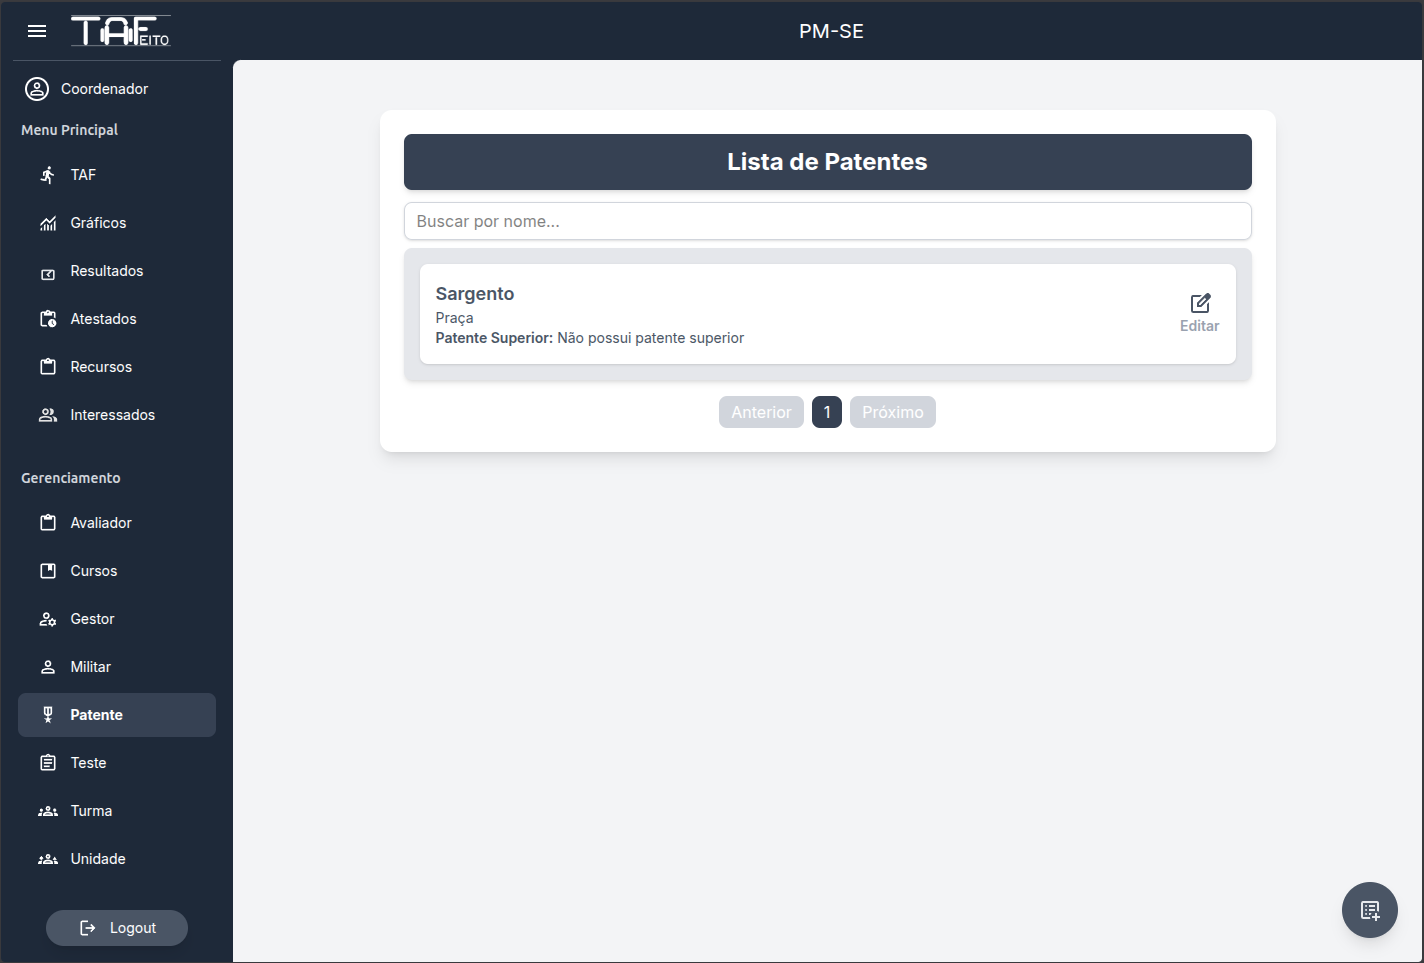
\includegraphics[scale=0.35]{./Imagens/tafeito/web/Patentes.png}
	\caption{Gerenciamento das Patentes}
	\label{fig:patentes}
\end{figure}

\begin{itemize}
	\item \label{item:gerenciar_cursos} \textbf{Gerenciamento dos Cursos}: disponível apenas para os Coordenadores e Gestores, seu objetivo é permitir o gerenciamento completo, desde visualização até edição de Cursos (\autoref{fig:cursos}). Também há um campo de pesquisa ativa, mecanismo idêntico ao da funcionalidade anterior, como também um botão no canto inferior direito que permite a adição de novos Cursos e, por fim, um botão com o nome "Editar" para permitir alterações. Aos Gestores é permitido apenas a visualização dos itens.
\end{itemize}

\begin{figure}[H]
	\centering
	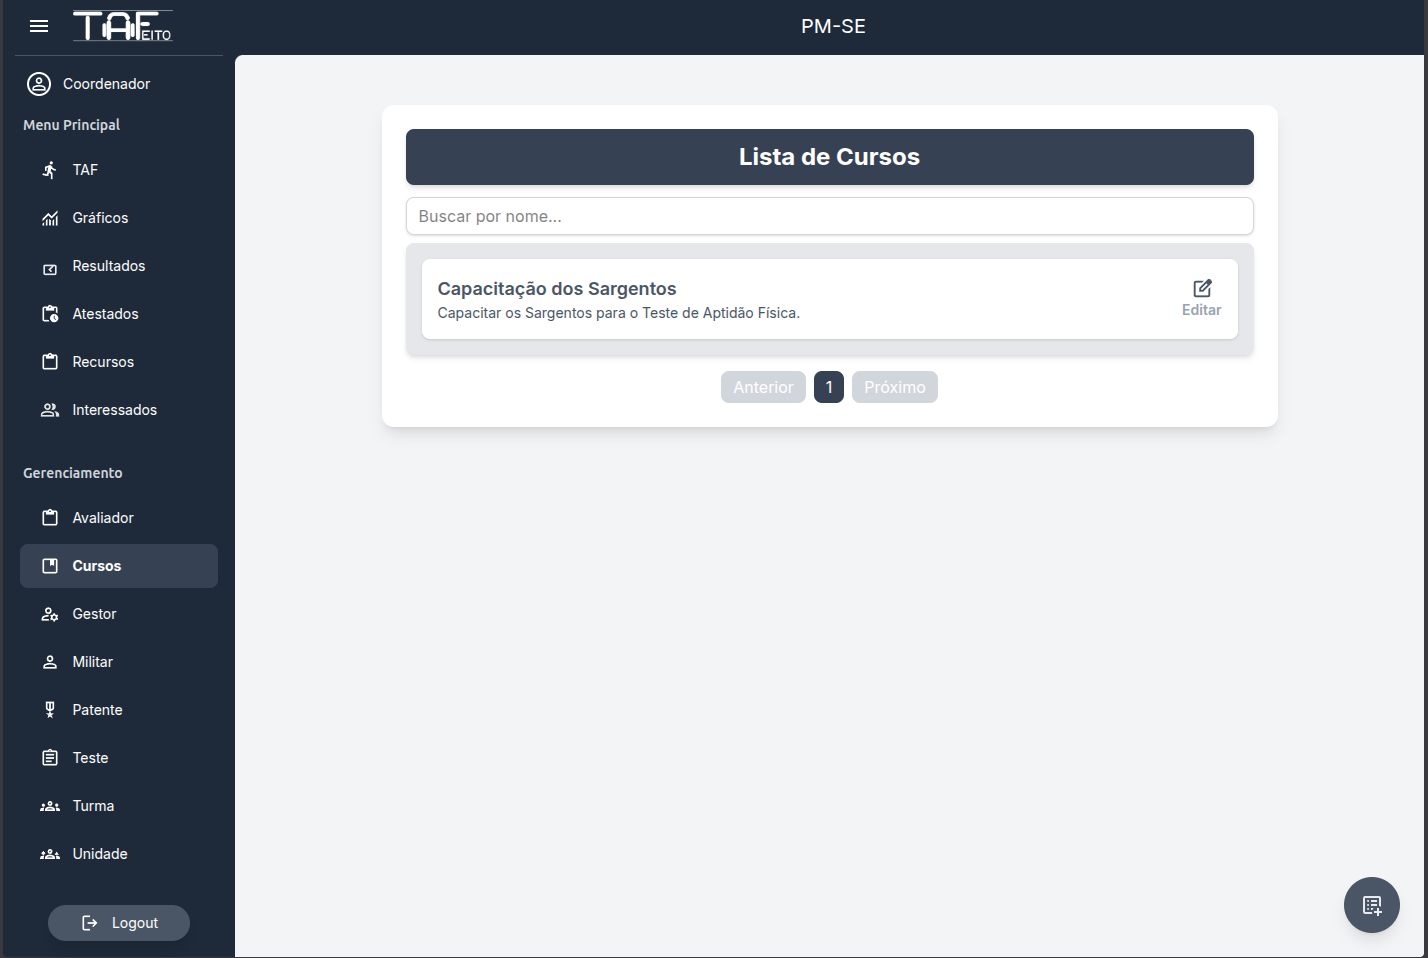
\includegraphics[scale=0.34]{./Imagens/tafeito/web/Cursos.png}
	\caption{Gerenciamento dos Cursos}
	\label{fig:cursos}
\end{figure}

\begin{itemize}
	\item \label{item:gerenciar_turmas} \textbf{Gerenciamento das Turmas}: disponível apenas para os Coordenadores e Gestores, seu objetivo é permitir o gerenciamento completo, desde visualização até edição de Turmas (\autoref{fig:turmas}). Também há um campo de pesquisa ativa, mecanismo idêntico ao da funcionalidade anterior, além de outros campos de pesquisa como "Ano", "Sequência Ano" e "Tipo", este sendo possível selecionar tipo Formação ou tipo Ingresso. Um botão para criação de novas Turmas também está presente no canto inferior direito, como também um botão para edição e, ao seu lado, um botão para visualização dos Militares inseridos nas Turmas. Métodos de criação e atualização não estão disponíveis para os Gestores.
\end{itemize}

\begin{figure}[H]
	\centering
	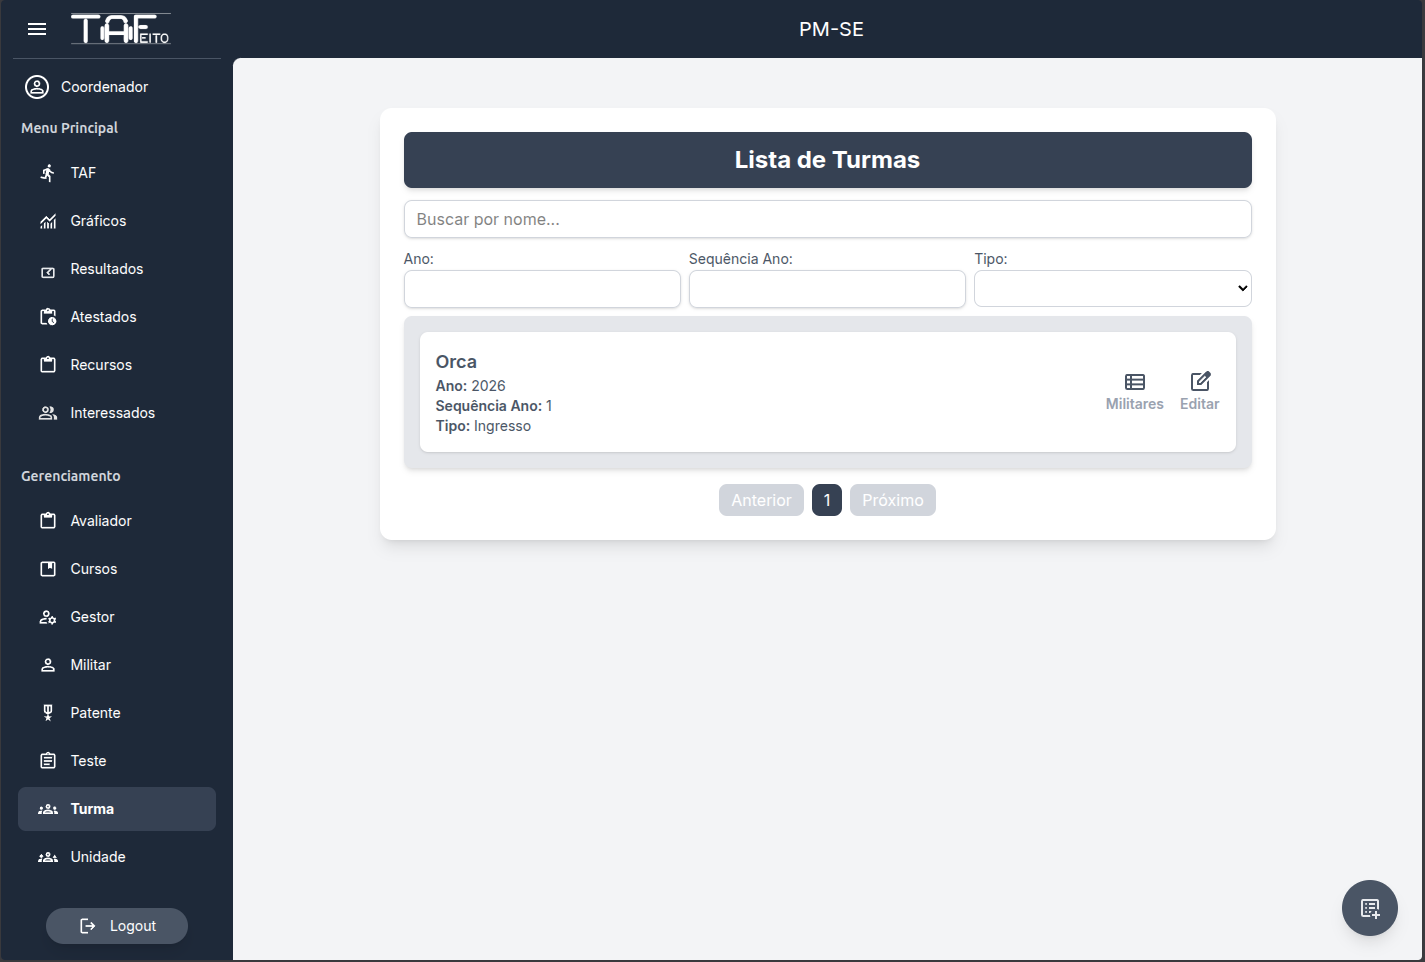
\includegraphics[scale=0.35]{./Imagens/tafeito/web/Turmas.png}
	\caption{Gerenciamento das Turmas}
	\label{fig:turmas}
\end{figure}

\begin{itemize}
	\item \label{item:gerenciar_militares} \textbf{Gerenciamento dos Militares}: disponível apenas para os Coordenadores e Gestores, seu objetivo é permitir o gerenciamento completo, desde visualização até edição de Turmas (\autoref{fig:militares}). Também há um campo de pesquisa ativa, mecanismo idêntico ao da funcionalidade anterior. Existem duas opções para o método de inserção de Militares, ambos localizados no canto inferior direito. O primeiro se refere à inserção individual, localizado à direita, onde o Coordenador conseguirá inserir as informações de apenas um único Militar, já o outro se refere à inserção múltipla, localizado à esquerda, onde o Coordenador conseguirá realizar o upload de uma planilha, em Excel, com as informações de mais de um Militar por linha. Um botão para permitir a edição de um Militar também estará disponível ao lado do seu nome. Gestores podem apenas visualizar os dados cadastrados.
\end{itemize}

\begin{figure}[H]
	\centering
	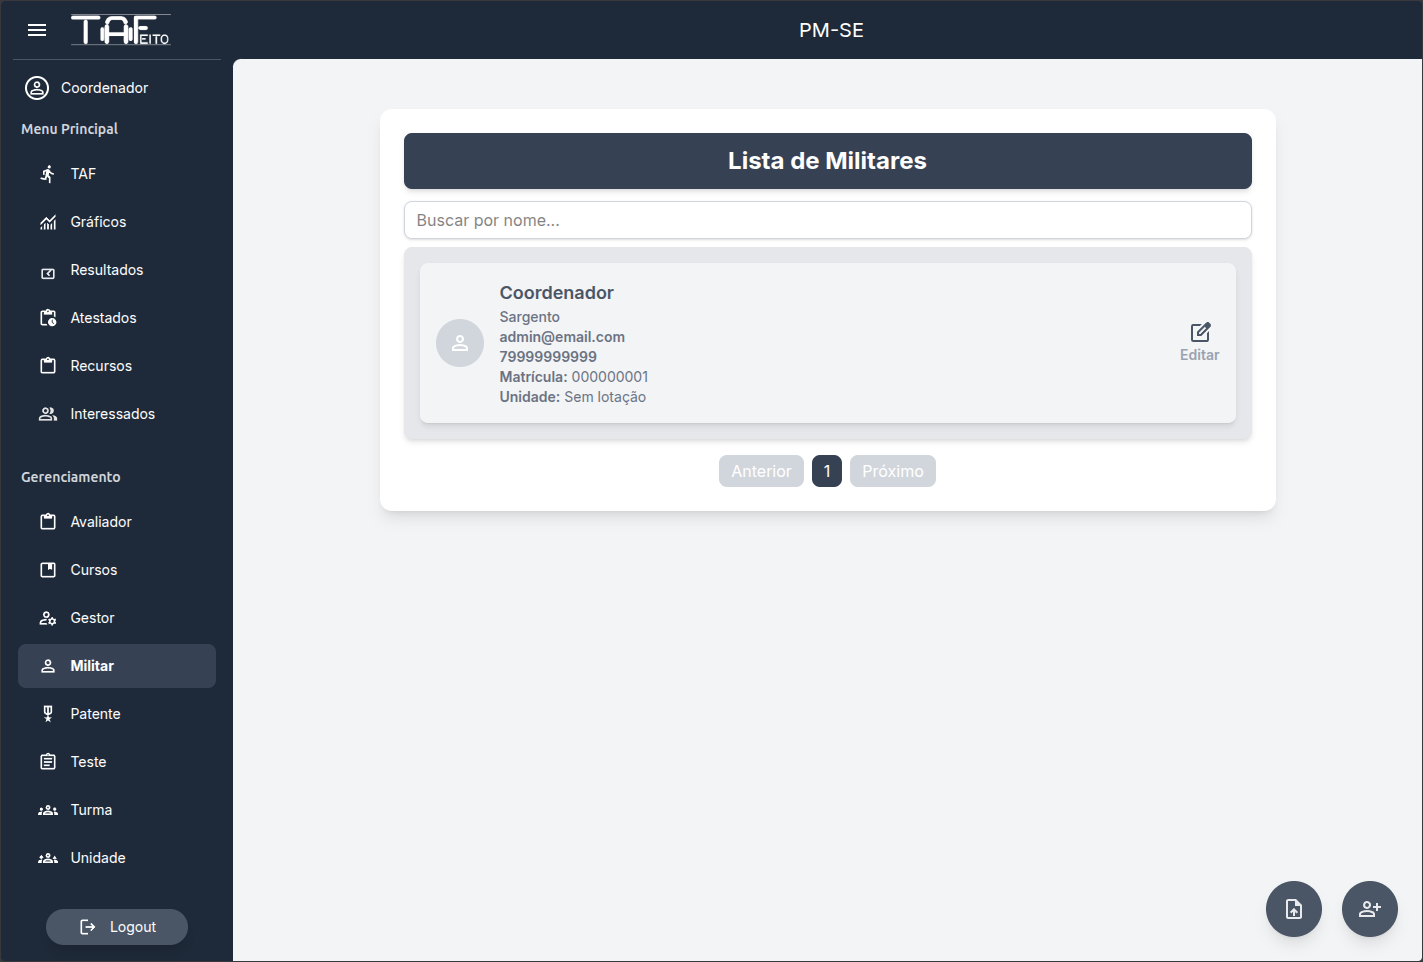
\includegraphics[scale=0.35]{./Imagens/tafeito/web/Militares.png}
	\caption{Gerenciamento dos Militares}
	\label{fig:militares}
\end{figure}

\begin{itemize}
	\item \label{item:gerenciar_unidades} \textbf{Gerenciamento das Unidades}: disponível apenas para os Coordenadores e Gestores, seu objetivo é permitir o gerenciamento completo, desde visualização até edição de Unidades (\autoref{fig:unidades}). Também há um campo de pesquisa ativa, mecanismo idêntico ao da funcionalidade anterior. Para cada unidade há duas opções de visualização, uma se refere a visualização de Militares inseridos e a outra está relacionada à visualização de Unidades que são subordinadas à atual, além de existir um botão para editar a referida Unidade. Os Gestores podem apenas visualizar os dados.
\end{itemize}

\begin{figure}[H]
	\centering
	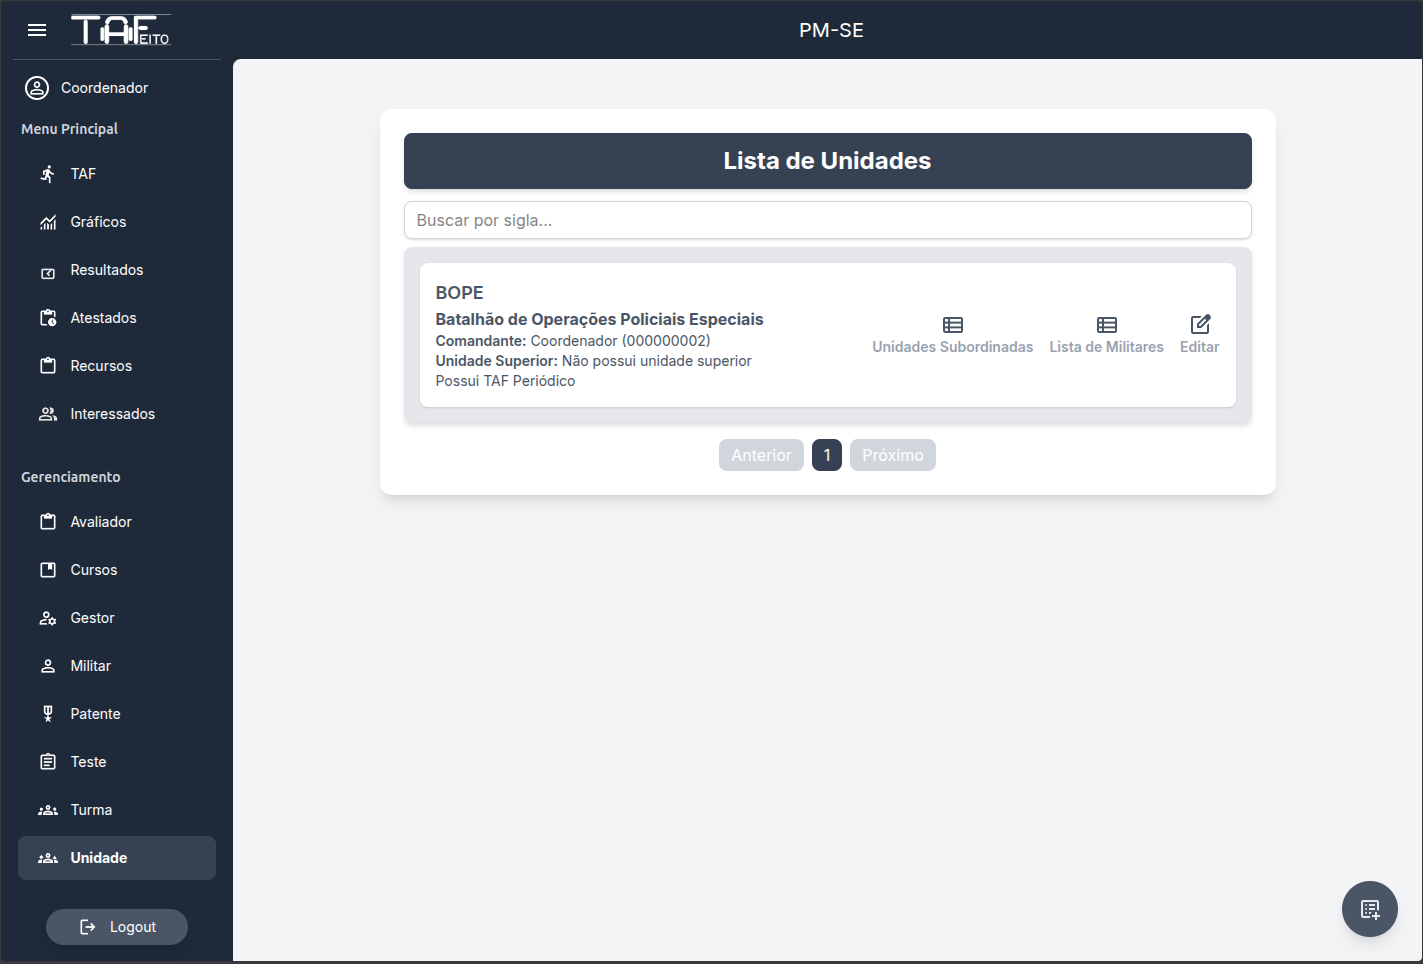
\includegraphics[scale=0.31]{./Imagens/tafeito/web/Unidades.png}
	\caption{Gerenciamento das Unidades}
	\label{fig:unidades}
\end{figure}

\begin{itemize}
	\item \label{item:gerenciar_testes} \textbf{Gerenciamento dos Testes}: disponível apenas para os Coordenadores e Gestores, seu objetivo é permitir o gerenciamento completo, desde visualização até edição de Testes (\autoref{fig:testes}). Também há um campo de pesquisa ativa com o mecanismo idêntico ao da funcionalidade anterior, porém, além do nome, também é possível pesquisar pelo gênero, masculino ou feminino, e pelo tipo da unidade exigida pelo teste, sendo distância, tempo ou repetição. Para cada Teste, também é permitido sua edição e, caso seja necessário adicionar mais Testes, um botão no canto inferior direito com o mecanismo de adição. Ao Gestor, cabe apenas a visualização dos dados.
\end{itemize}

\begin{figure}[H]
	\centering
	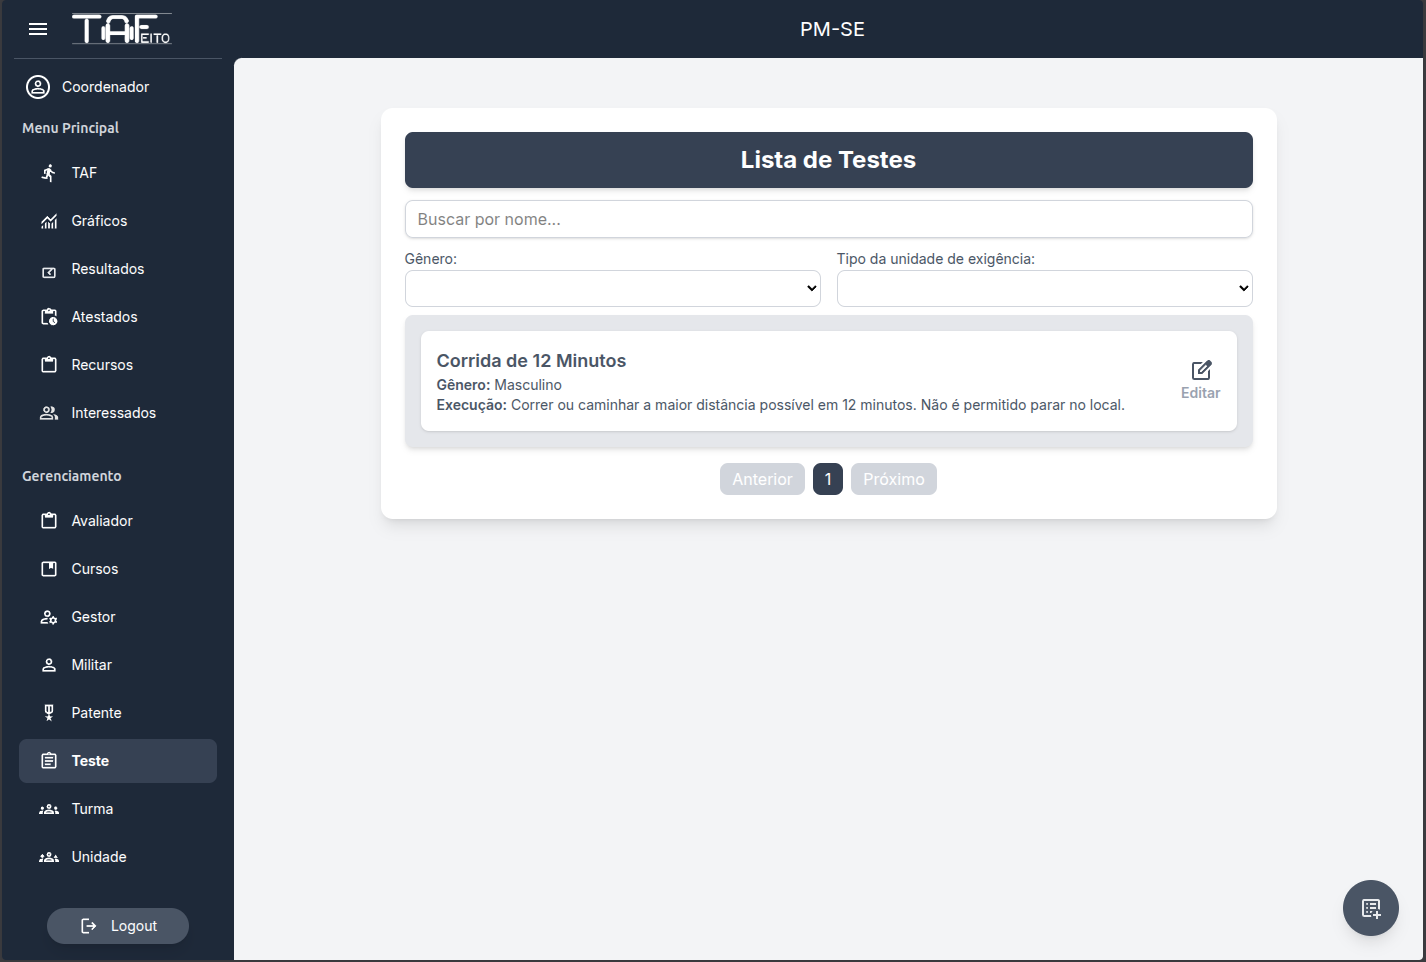
\includegraphics[scale=0.35]{./Imagens/tafeito/web/Testes.png}
	\caption{Gerenciamento dos Testes}
	\label{fig:testes}
\end{figure}

\begin{itemize}
	\item \label{item:gerenciar_tafs} \textbf{Gerenciamento dos TAFs}: disponível apenas para os Coordenadores e Gestores, seu objetivo é permitir o gerenciamento completo, desde visualização até edição dos TAFs (\autoref{fig:tafs}). Há a presença do campo de pesquisa por nome, com o mecanismo de busca idêntico ao já citado anteriormente, como também data de início, data de término, tipo do TAF, tipo da Patente, status e pela matrícula do Coordenador. Para cada TAF é permitido sua edição, visualização dos Grupos, onde há a presença dos Militares e Avaliadores, visualização dos Testes e, por fim, o edital daquele TAF. Para cadastrar novos TAFs, há a presença do botão no canto inferior direito, igual às demais funcionalidades. Ao Gestor fica disponível apenas a visualização dos dados inseridos.
\end{itemize}

\begin{figure}[H]
	\centering
	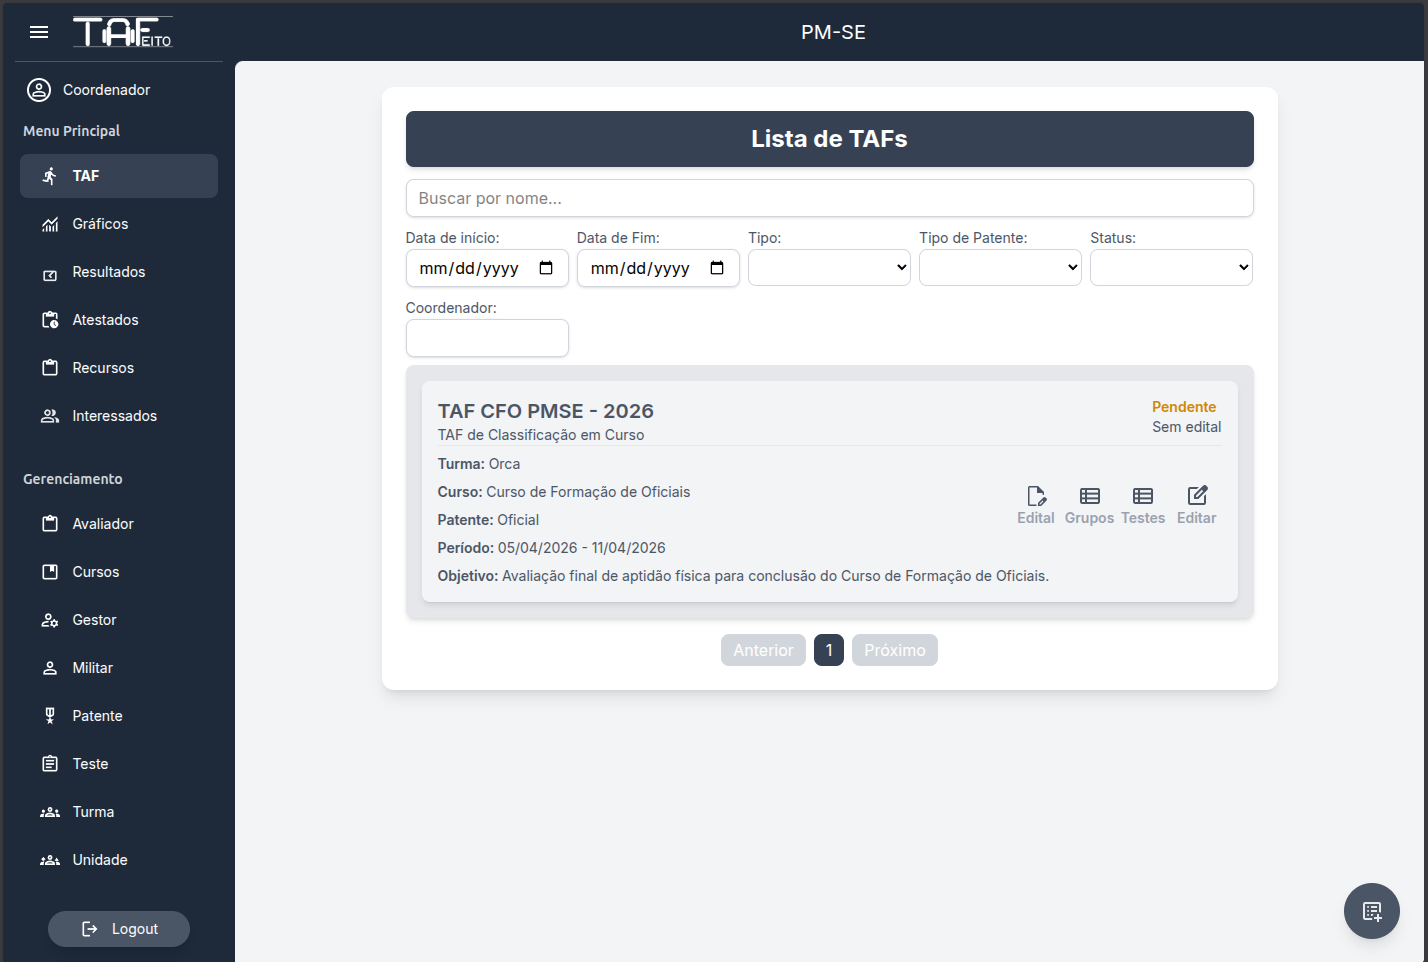
\includegraphics[scale=0.294]{./Imagens/tafeito/web/TAFs.png}
	\caption{Gerenciamento dos TAFs}
	\label{fig:tafs}
\end{figure}

\begin{itemize}
	\item \label{item:gerenciar_avaliadores} \textbf{Gerenciamento dos Avaliadores}: disponível apenas para os Coordenadores e Gestores, seu objetivo é permitir que Militares recebam e percam o papel de Avaliador, além de atribuí-los aos TAFs (\autoref{fig:avaliadores}). Há a presença do campo de pesquisa por nomes dos Avaliadores, com o mecanismo de busca idêntico ao já citado anteriormente, além de botões para atribuir o Avaliador a um TAF ou realizar sua remoção do papel. Caso seja necessário adicionar novos Avaliadores, há um botão no canto inferior direito para esse mecanismo. O Gestor possui apenas a função de visualização dos dados.
\end{itemize}

\begin{figure}[H]
	\centering
	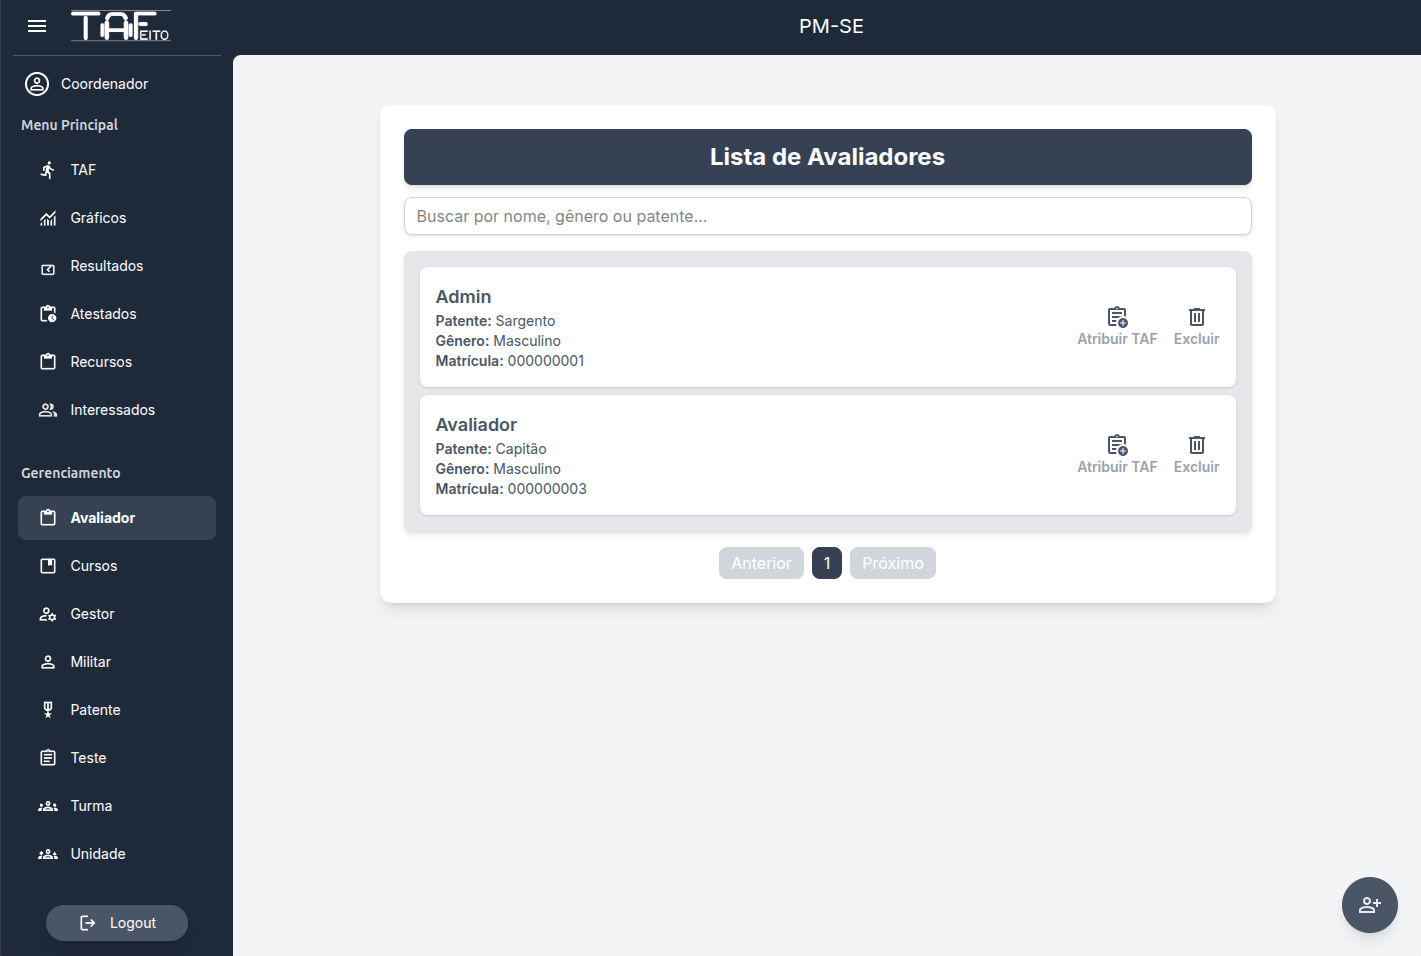
\includegraphics[scale=0.35]{./Imagens/tafeito/web/Avaliadores.png}
	\caption{Gerenciamento dos Avaliadores}
	\label{fig:avaliadores}
\end{figure}

\begin{itemize}
	\item \label{item:resultados} \textbf{Resultados dos TAFs}: disponível apenas para os Coordenadores e Gestores, seu objetivo é permitir a visualização dos resultados dos TAFs (\autoref{fig:tafs}), contendo informações da quantidade de Militares presentes no TAF, quantos se tornaram aptos, ou seja, atingiu a pontuação exigida durante a criação do TAF, quantos estão pendentes dos resultados e aqueles que não obtiveram a pontuação mínima exigida. Além disso, é possível visualizar o resultado de cada Militar e qual sua posição. Também é possível visualizar os Grupos presentes e realizar o Download, em PDF, do resultado deste TAF.
\end{itemize}

\begin{figure}[H]
	\centering
	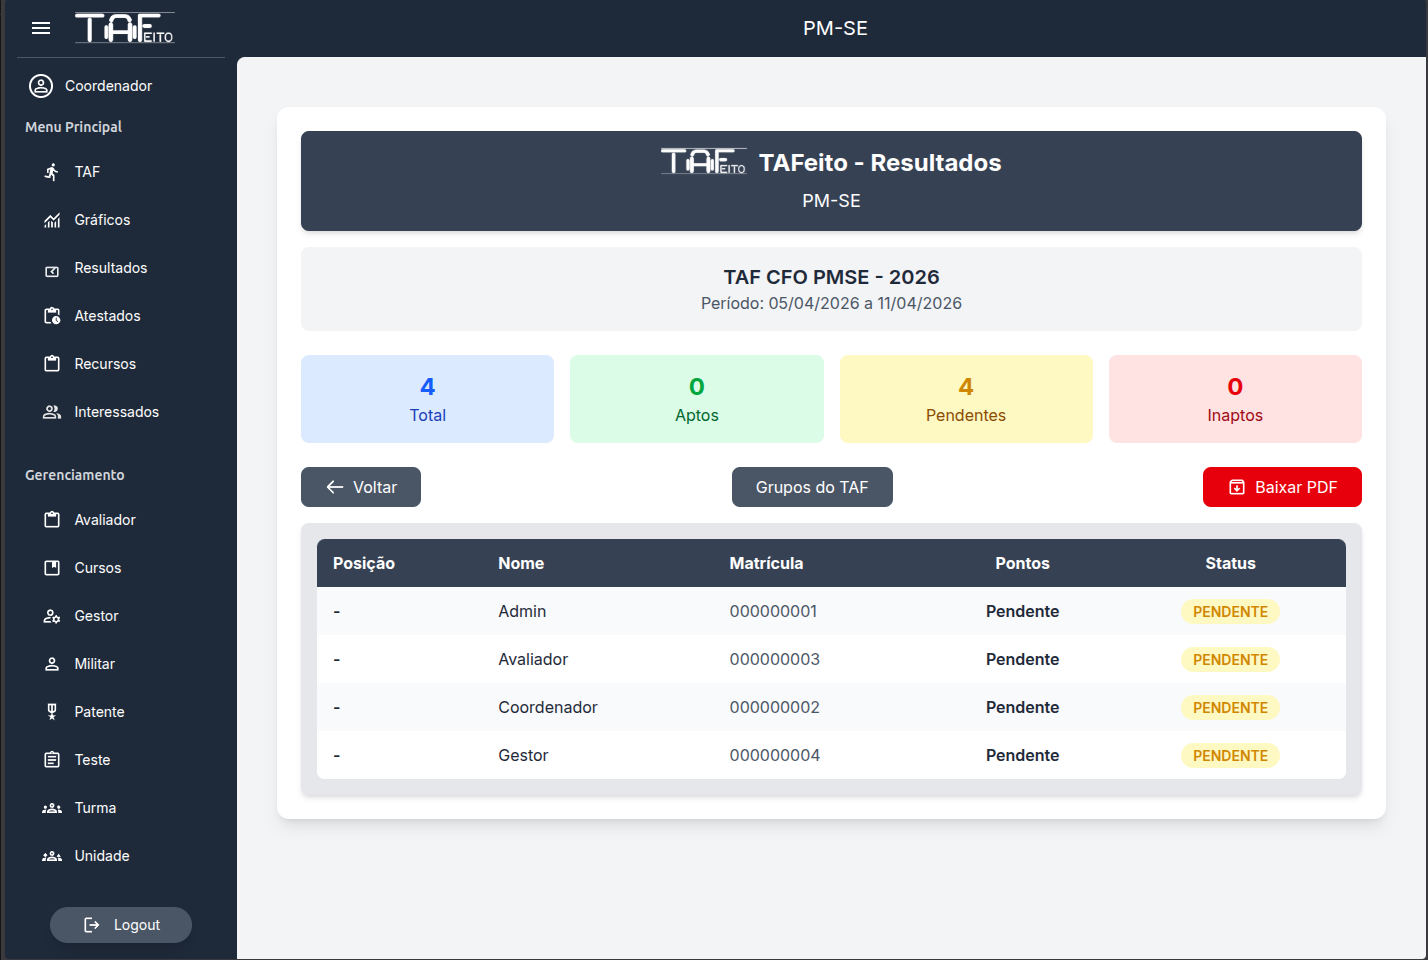
\includegraphics[scale=0.29]{./Imagens/tafeito/web/Resultados.png}
	\caption{Resultados dos TAFs}
	\label{fig:resultados}
\end{figure}

\begin{itemize}
	\item \label{item:recursos} \textbf{Recursos dos TAFs}: disponível apenas para os Coordenadores e Gestores, seu objetivo é permitir a visualização e aprovação/reprovação dos Recursos dos TAFs (\autoref{fig:recursos}), podendo visualizar seu motivo. O perfil Gestor apenas visualiza os dados inseridos.
\end{itemize}

\begin{figure}[H]
	\centering
	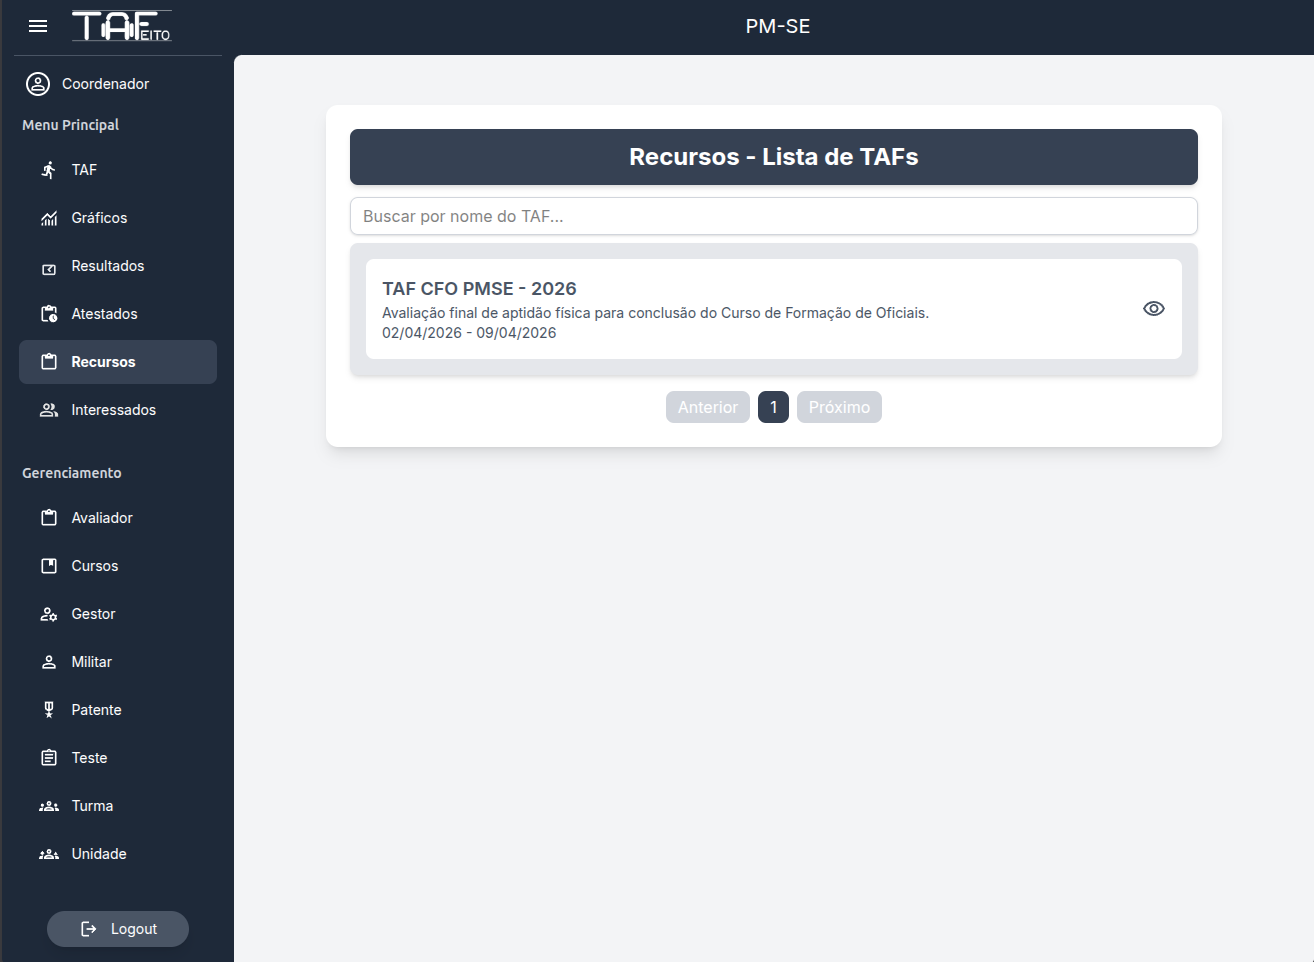
\includegraphics[scale=0.28]{./Imagens/tafeito/web/Recursos.png}
	\caption{Recursos dos TAFs}
	\label{fig:recursos}
\end{figure}

\begin{itemize}
	\item \label{item:atestados} \textbf{Atestados dos TAFs}: disponível apenas para os Coordenadores e Gestores, seu objetivo é permitir a visualização e aprovação/reprovação dos Atestados dos TAFs (\autoref{fig:atestados}), possuindo a mesma operação vista na funcionalidade de Recursos. Os Gestores conseguem apenas visualizar os atestados.
\end{itemize}

\begin{figure}[H]
	\centering
	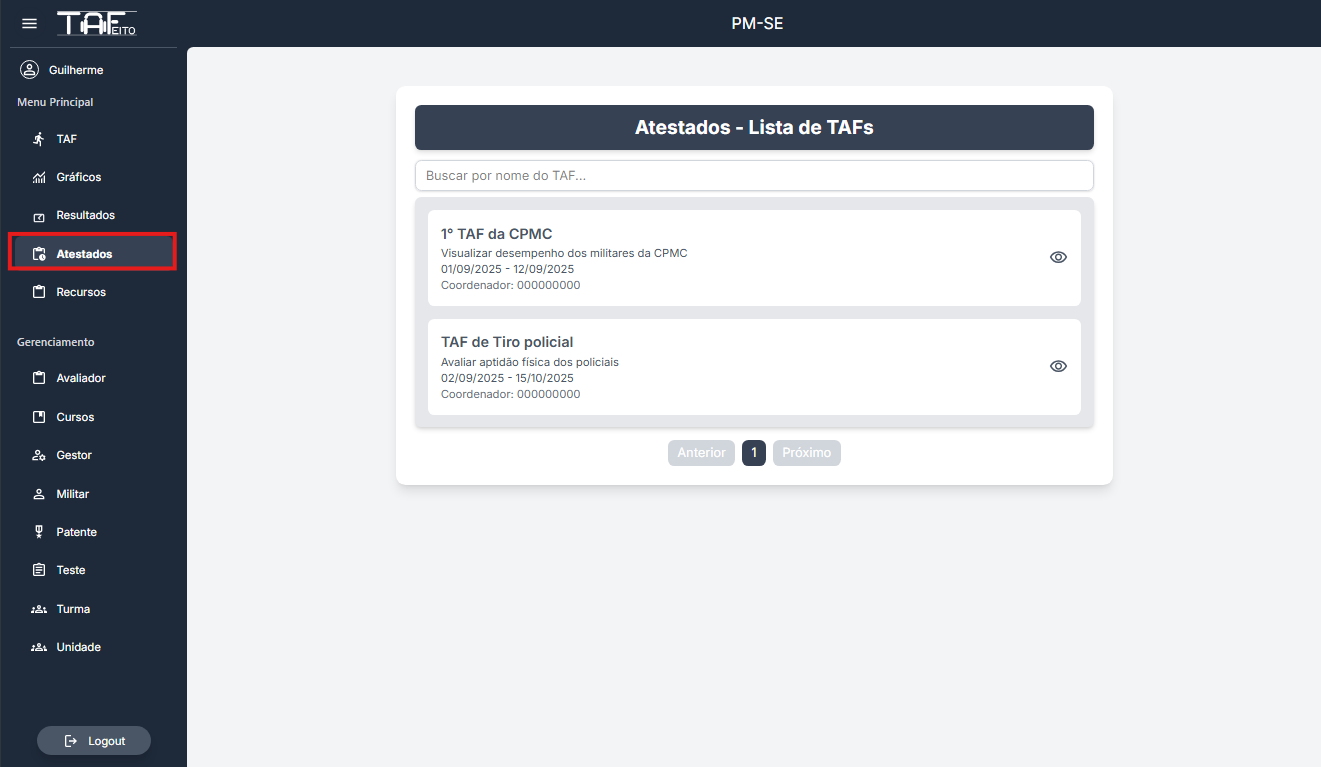
\includegraphics[scale=0.3]{./Imagens/tafeito/web/Atestados.png}
	\caption{Atestados dos TAFs}
	\label{fig:atestados}
\end{figure}

\begin{itemize}
	\item \label{item:interesses} \textbf{Interessados nos TAFs}: disponível apenas para os Coordenadores, seu objetivo é permitir a aprovação/reprovação dos Militares que demonstraram interesse no TAF (\autoref{fig:interessados}), possuindo a mesma operação vista na funcionalidade de Recursos (\autoref{fig:demonstracao_interesse}).
\end{itemize}

\begin{figure}[H]
	\centering
	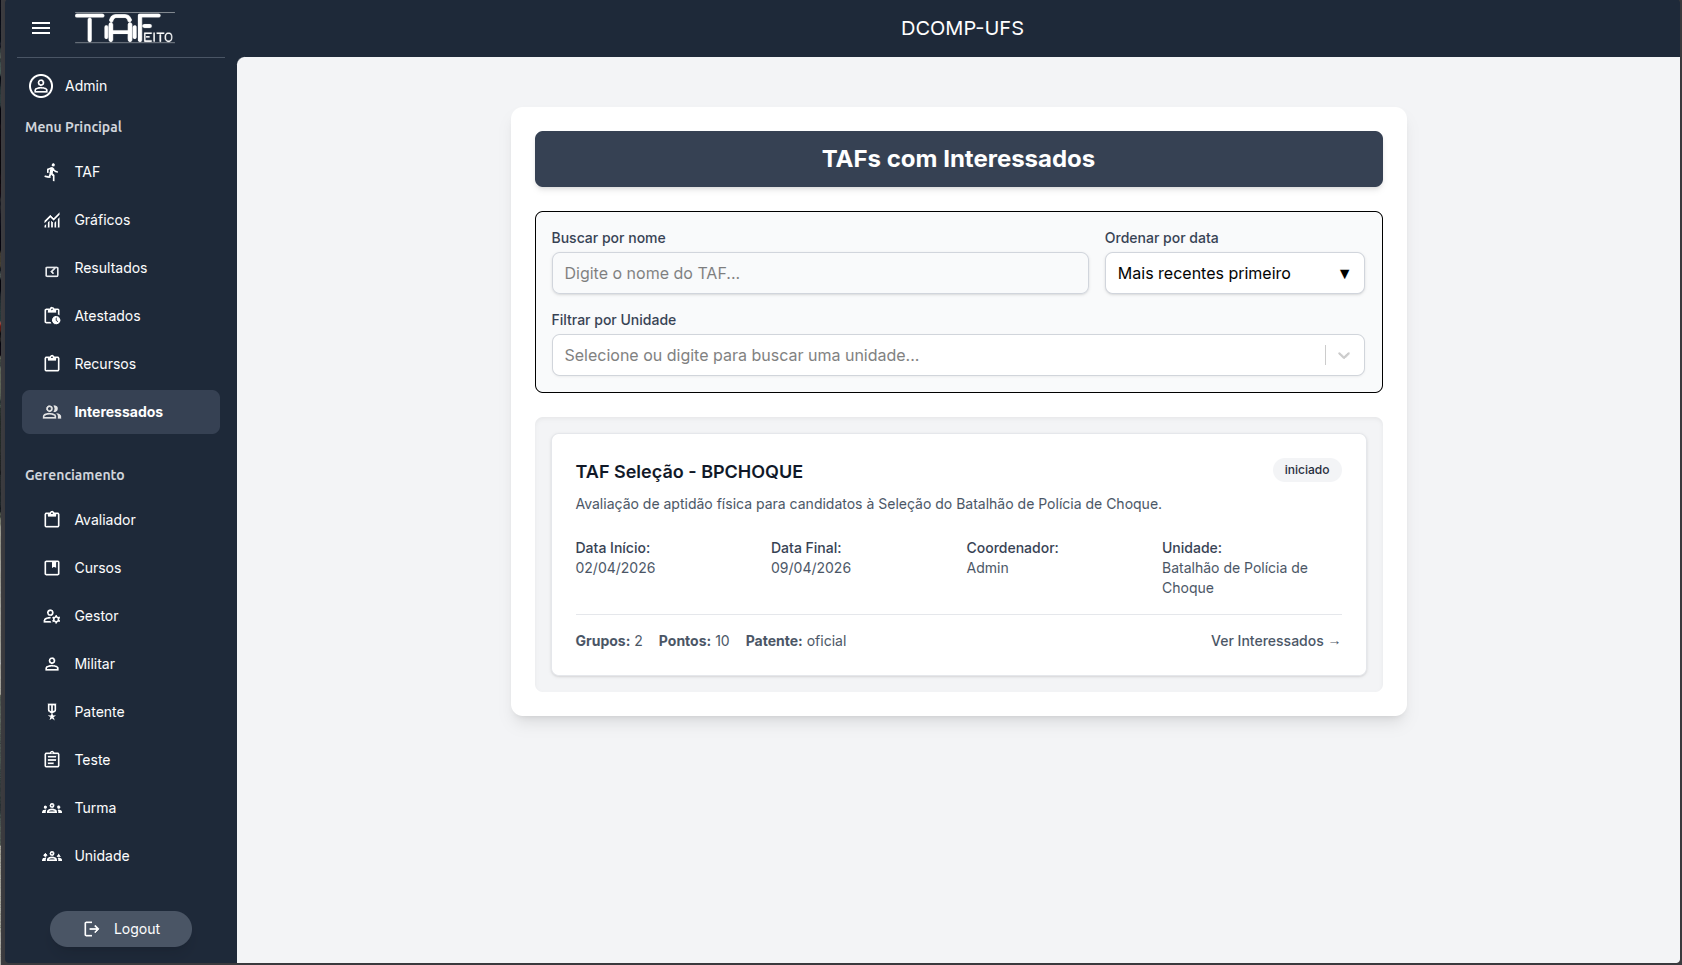
\includegraphics[scale=0.27]{./Imagens/tafeito/web/Interessados.png}
	\caption{Interessados nos TAFs}
	\label{fig:interessados}
\end{figure}

\begin{figure}[H]
	\centering
	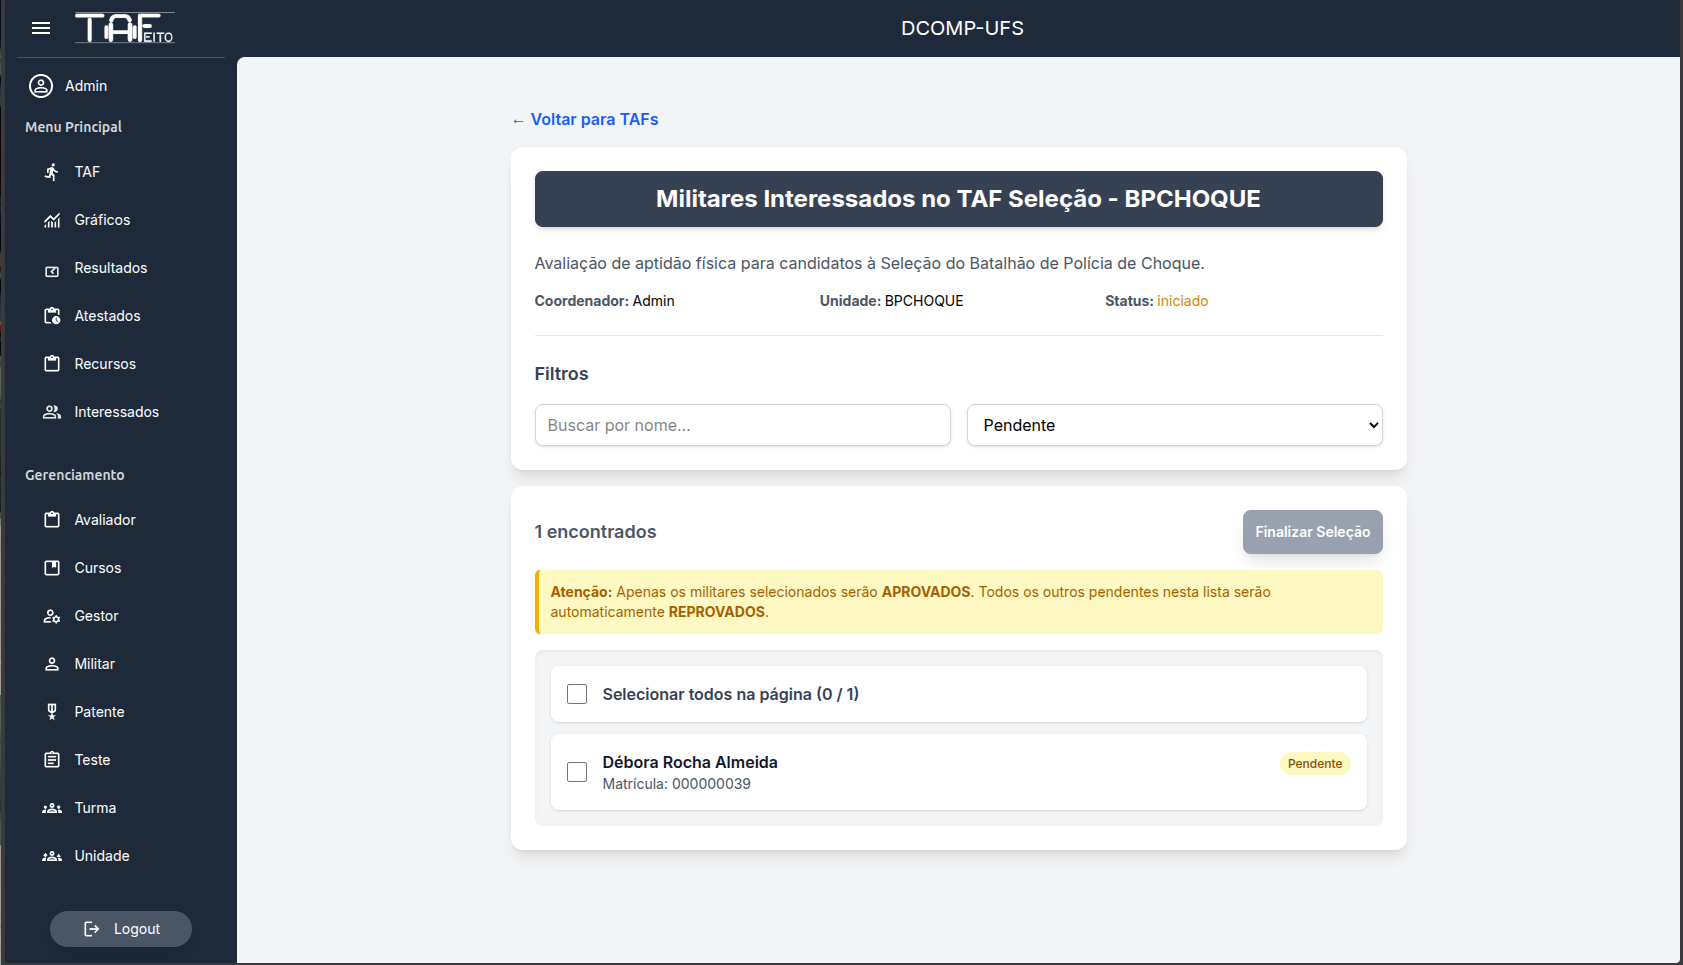
\includegraphics[scale=0.27]{./Imagens/tafeito/web/DemonstraInteresse.png}
	\caption{Demonstração de Interesse no TAF}
	\label{fig:demonstracao_interesse}
\end{figure}

\begin{itemize}
	\item \textbf{Taxa de Aprovação por Turma}: funcionalidade de gráfico vista por Coordenadores e Gestores cujo objetivo é mostrar a taxa de aprovação de um TAF aplicado a uma Turma (\autoref{fig:taxa_aprovacao_turma}), sendo uma funcionalidade exclusivamente de visualização. Nela, é possível mostrar a taxa ao selecionar, no canto esquerdo, a turma desejada, mostrando o resultado após isso. A taxa é calculada pela divisão do total de Militares aptos com a quantidade de Militares presentes na Turma.
\end{itemize}

\begin{figure}[H]
	\centering
	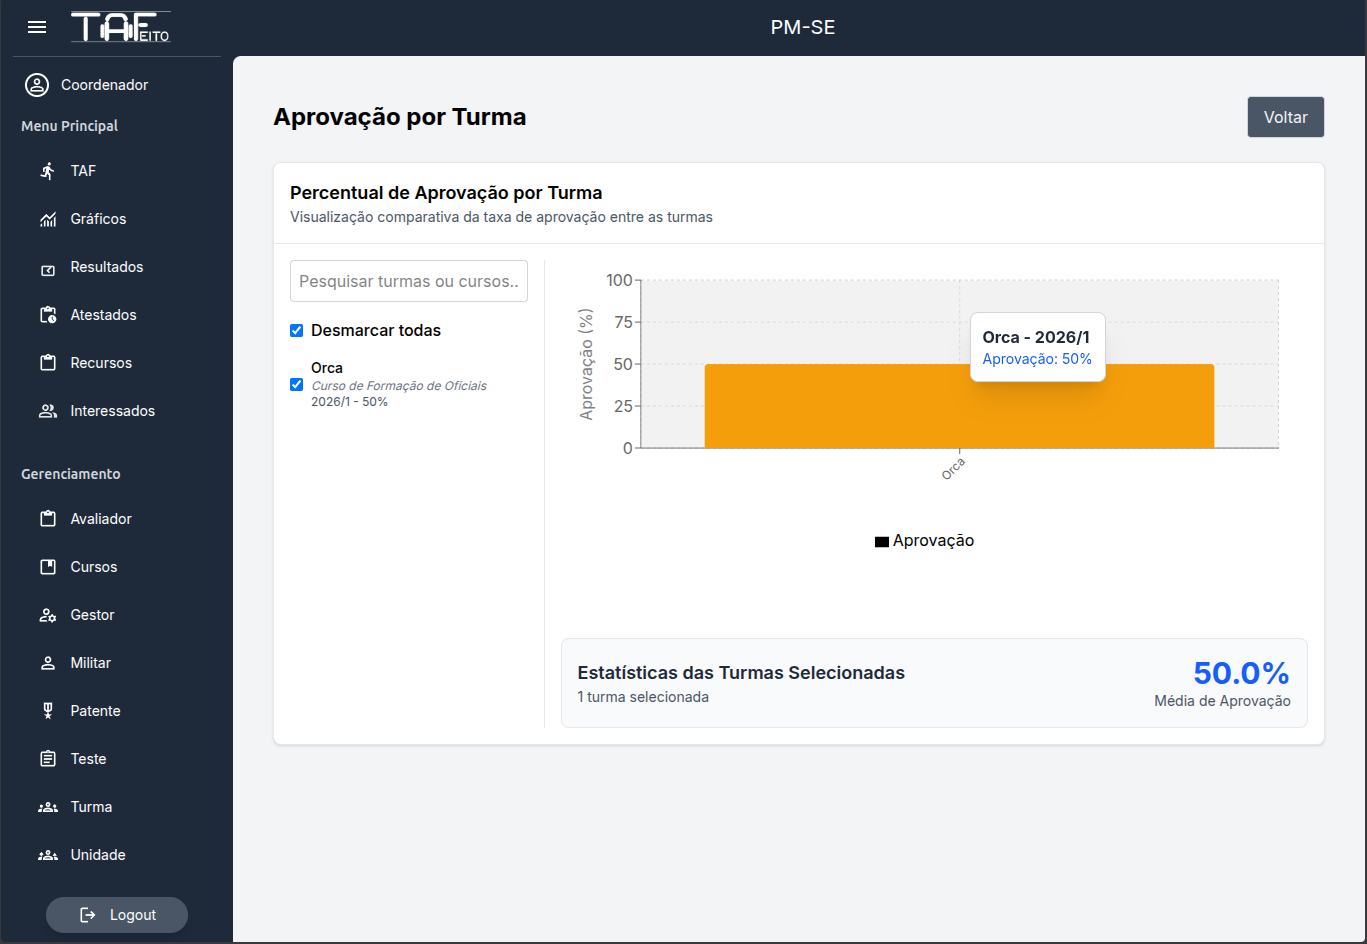
\includegraphics[scale=0.3]{./Imagens/tafeito/web/TaxaAprovacaoTurma.png}
	\caption{Taxa de Aprovação por Turma}
	\label{fig:taxa_aprovacao_turma}
\end{figure}

\begin{itemize}
	\item \textbf{Média de Pontuação por Turma}: funcionalidade de gráfico vista por Coordenadores e Gestores cujo objetivo é mostrar a média de pontuação de um TAF aplicado a uma Turma (\autoref{fig:media_pontuacao_turma}), sendo uma funcionalidade exclusivamente de visualização. Nela, é possível mostrar a média selecionando, no canto esquerdo da funcionalidade, a turma desejada, mostrando o resultado após isso. A média é calculada por meio da divisão do total de pontos obtidos pela turma com a quantidade de Militares presentes nesta turma.
\end{itemize}

\begin{figure}[H]
	\centering
	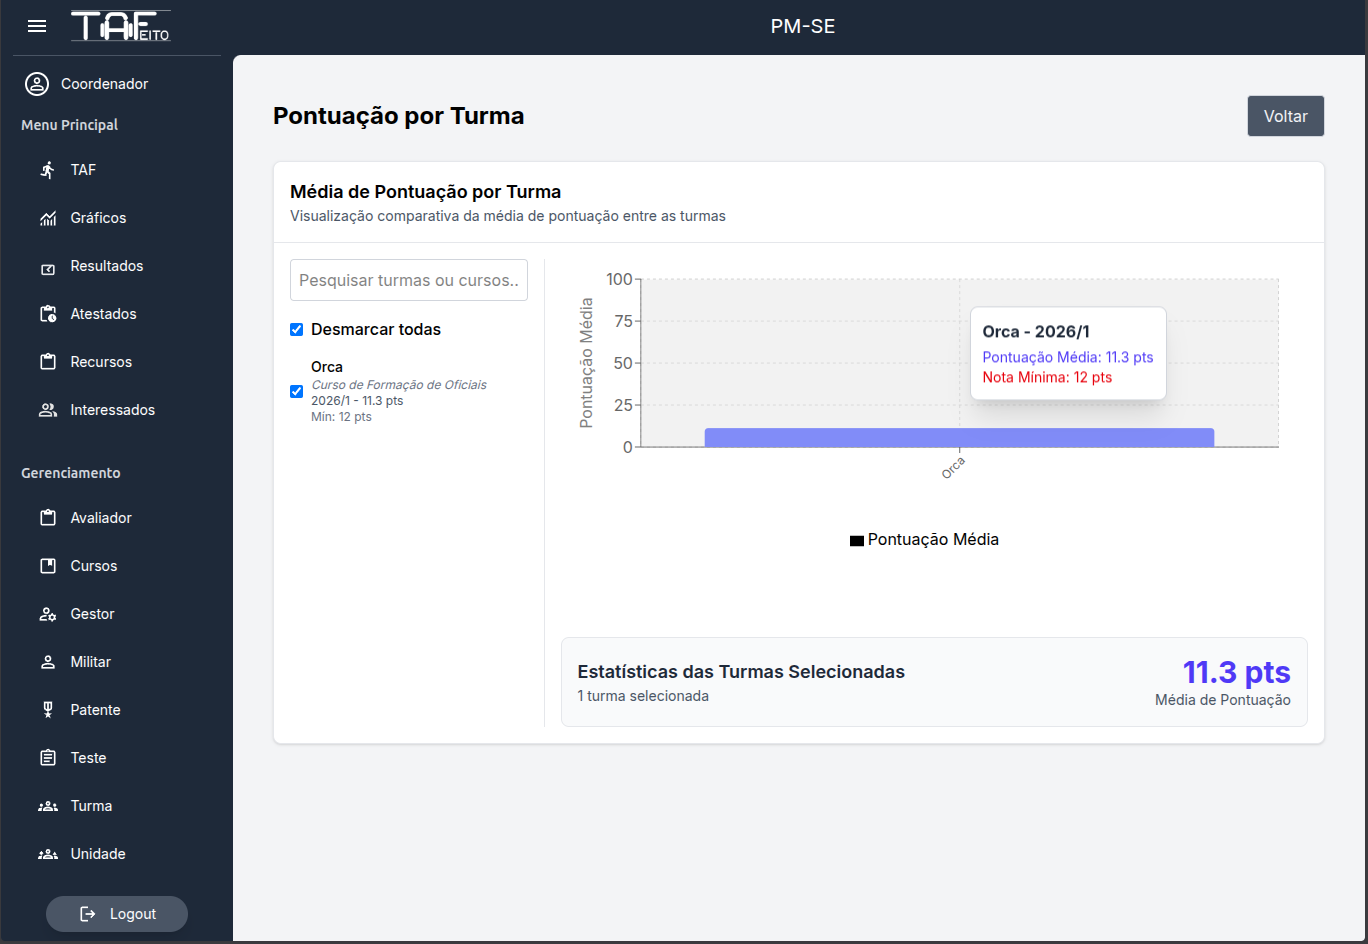
\includegraphics[scale=0.3]{./Imagens/tafeito/web/MediaPontuacaoTurma.png}
	\caption{Média de Pontuação por Turma}
	\label{fig:media_pontuacao_turma}
\end{figure}

\begin{itemize}
	\item \textbf{Taxa de Aprovação por Unidade}: funcionalidade de gráfico vista por Coordenadores e Gestores cujo objetivo é mostrar a taxa de aprovação de um TAF aplicado a uma Unidade, podendo ser um TAF Periódico (\autoref{fig:taxa_aprovacao_unidade_periodico}) ou um TAF para ingressão em Unidade (\autoref{fig:taxa_aprovacao_unidade_ingresso}), onde ambos tipos possuem a mesma estrutura para o gráfico de Taxa de Aprovação, com o adicional de seleção do período da aplicação do TAF, também localizado no lado esquerdo.
\end{itemize}

\begin{figure}[H]
	\centering
	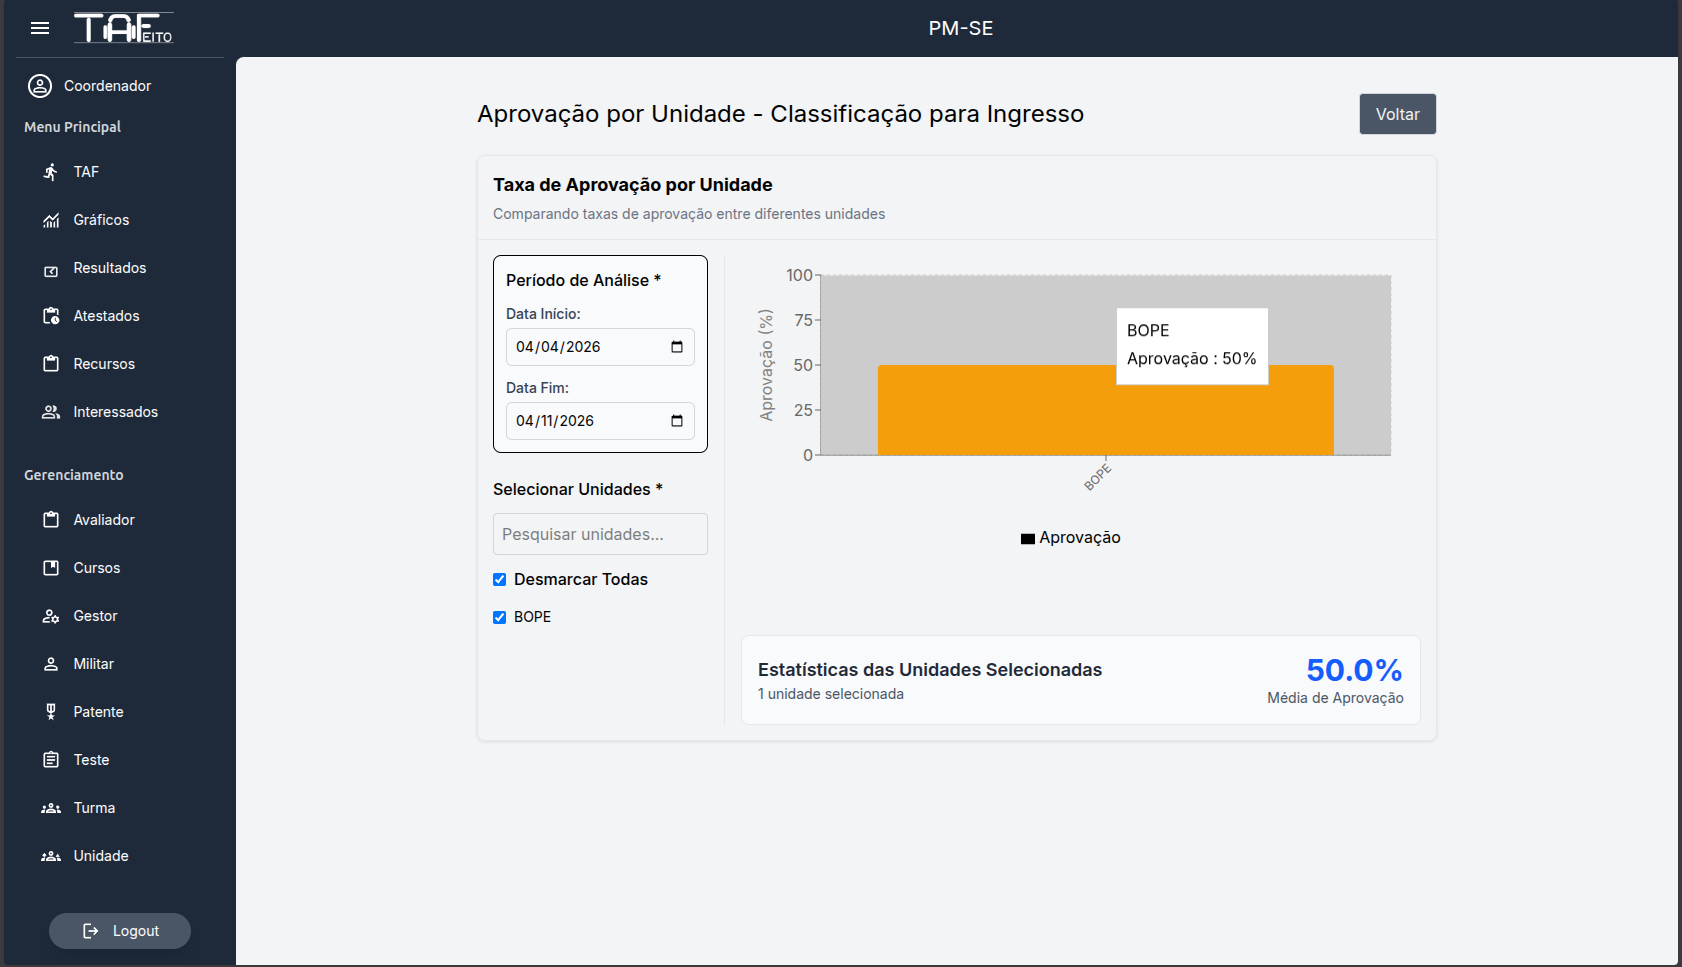
\includegraphics[scale=0.27]{./Imagens/tafeito/web/TaxaAprovacaoUnidadePeriodico.png}
	\caption{Taxa de Aprovação por Unidade Periódico}
	\label{fig:taxa_aprovacao_unidade_periodico}
\end{figure}

\begin{figure}[H]
	\centering
	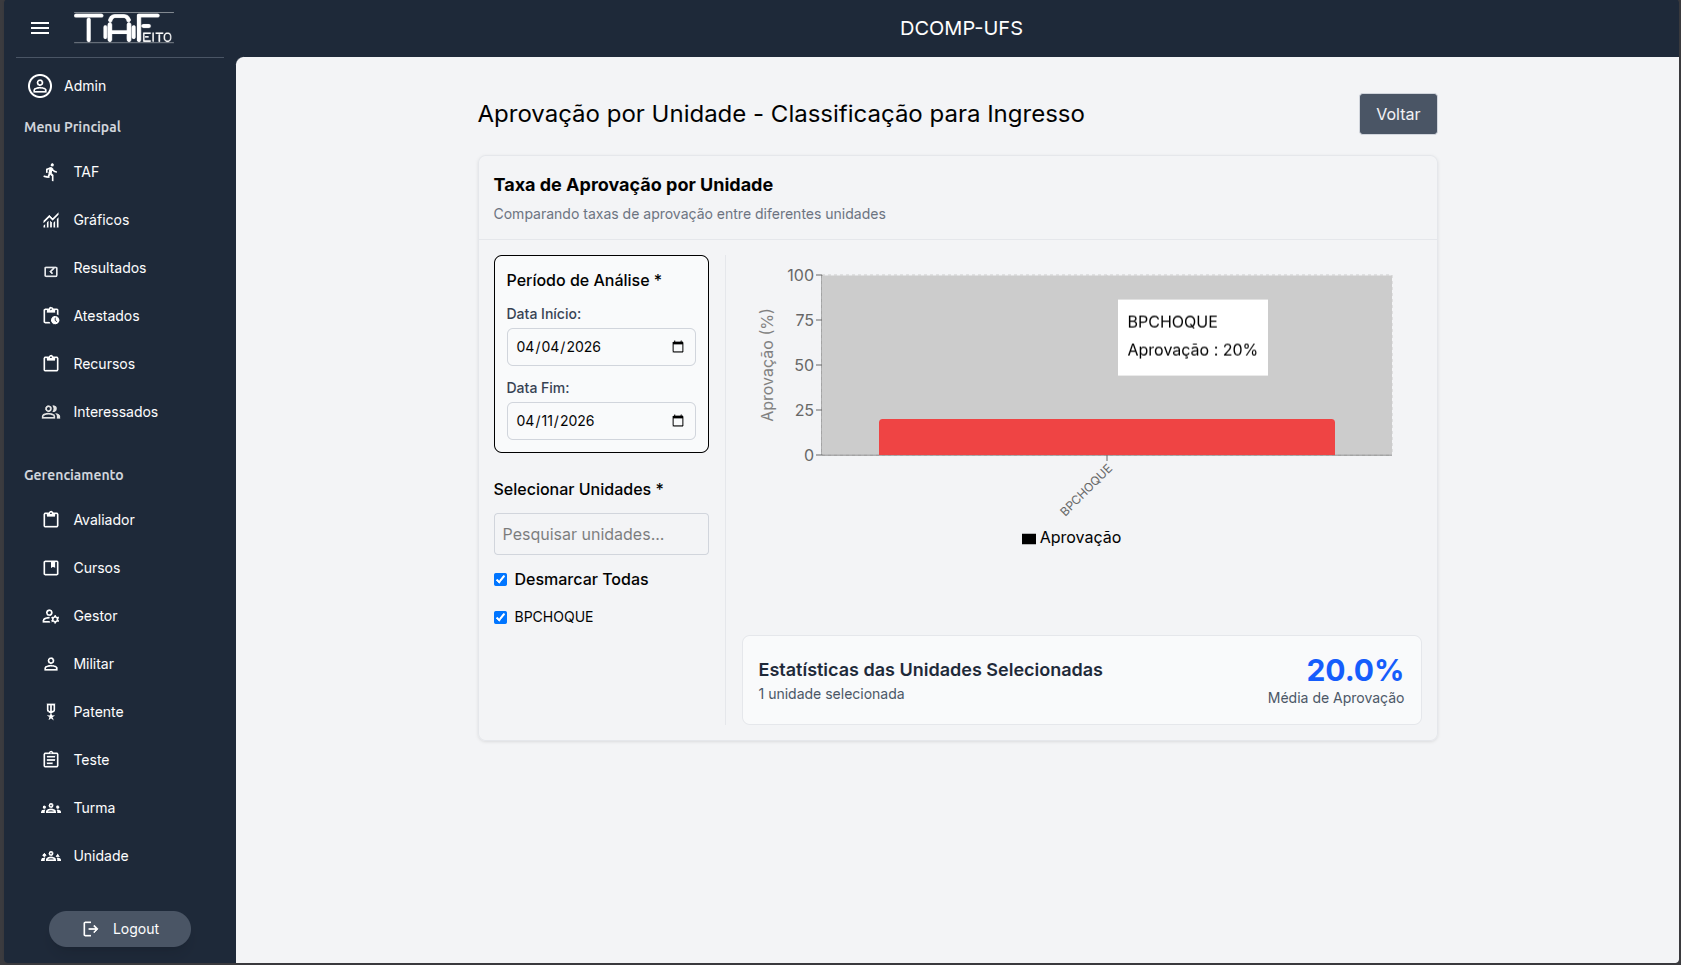
\includegraphics[scale=0.27]{./Imagens/tafeito/web/TaxaAprovacaoUnidadeIngresso.png}
	\caption{Taxa de Aprovação por Unidade Ingresso}
	\label{fig:taxa_aprovacao_unidade_ingresso}
\end{figure}

\begin{itemize}
	\item \textbf{Média de Pontuação por Unidade}: funcionalidade de gráfico vista por Coordenadores e Gestores cujo objetivo é mostrar a média de pontuação de um TAF aplicado a uma Unidade, podendo ser um TAF Periódico (\autoref{fig:media_pontuacao_unidade_periodico}) ou um TAF para ingressão em Unidade (\autoref{fig:media_pontuacao_unidade_ingresso}), onde, por ser um TAF aplicado à uma Unidade, é necessário, em ambos, selecionar o período de aplicação do TAF e a Unidade desejada para exibição dos resultados.
\end{itemize}

\begin{figure}[H]
	\centering
	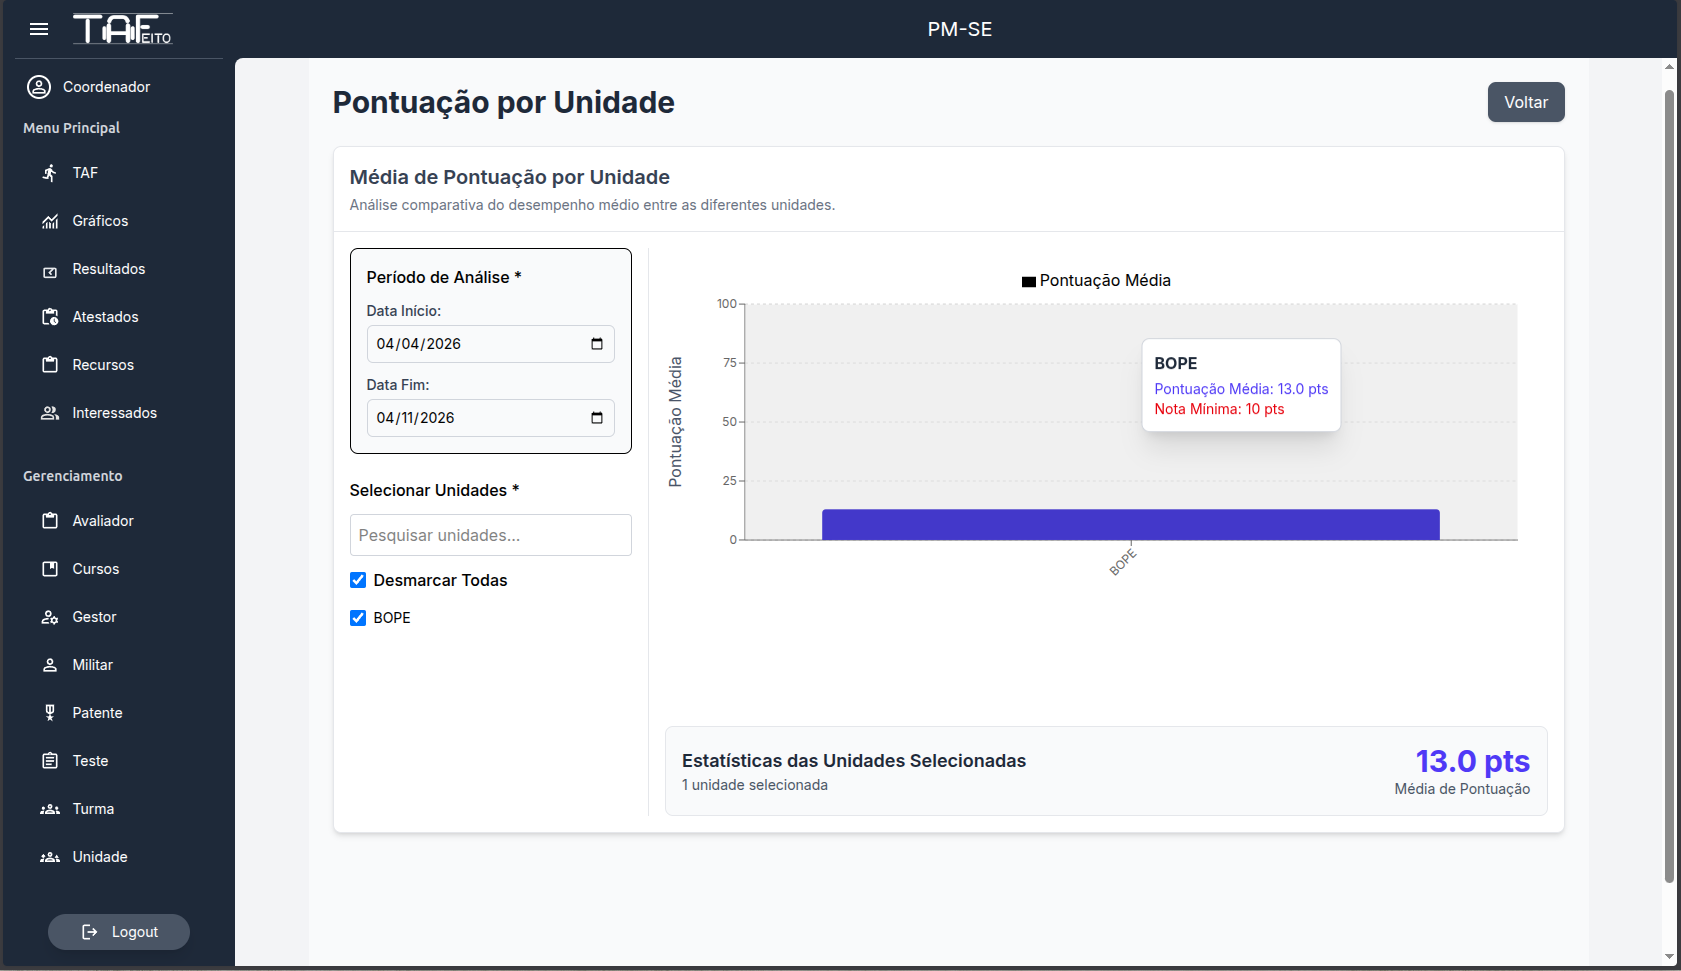
\includegraphics[scale=0.27]{./Imagens/tafeito/web/MediaPontuacaoUnidadePeriodico.png}
	\caption{Média de Pontuação por Unidade Periódico}
	\label{fig:media_pontuacao_unidade_periodico}
\end{figure}

\begin{figure}[H]
	\centering
	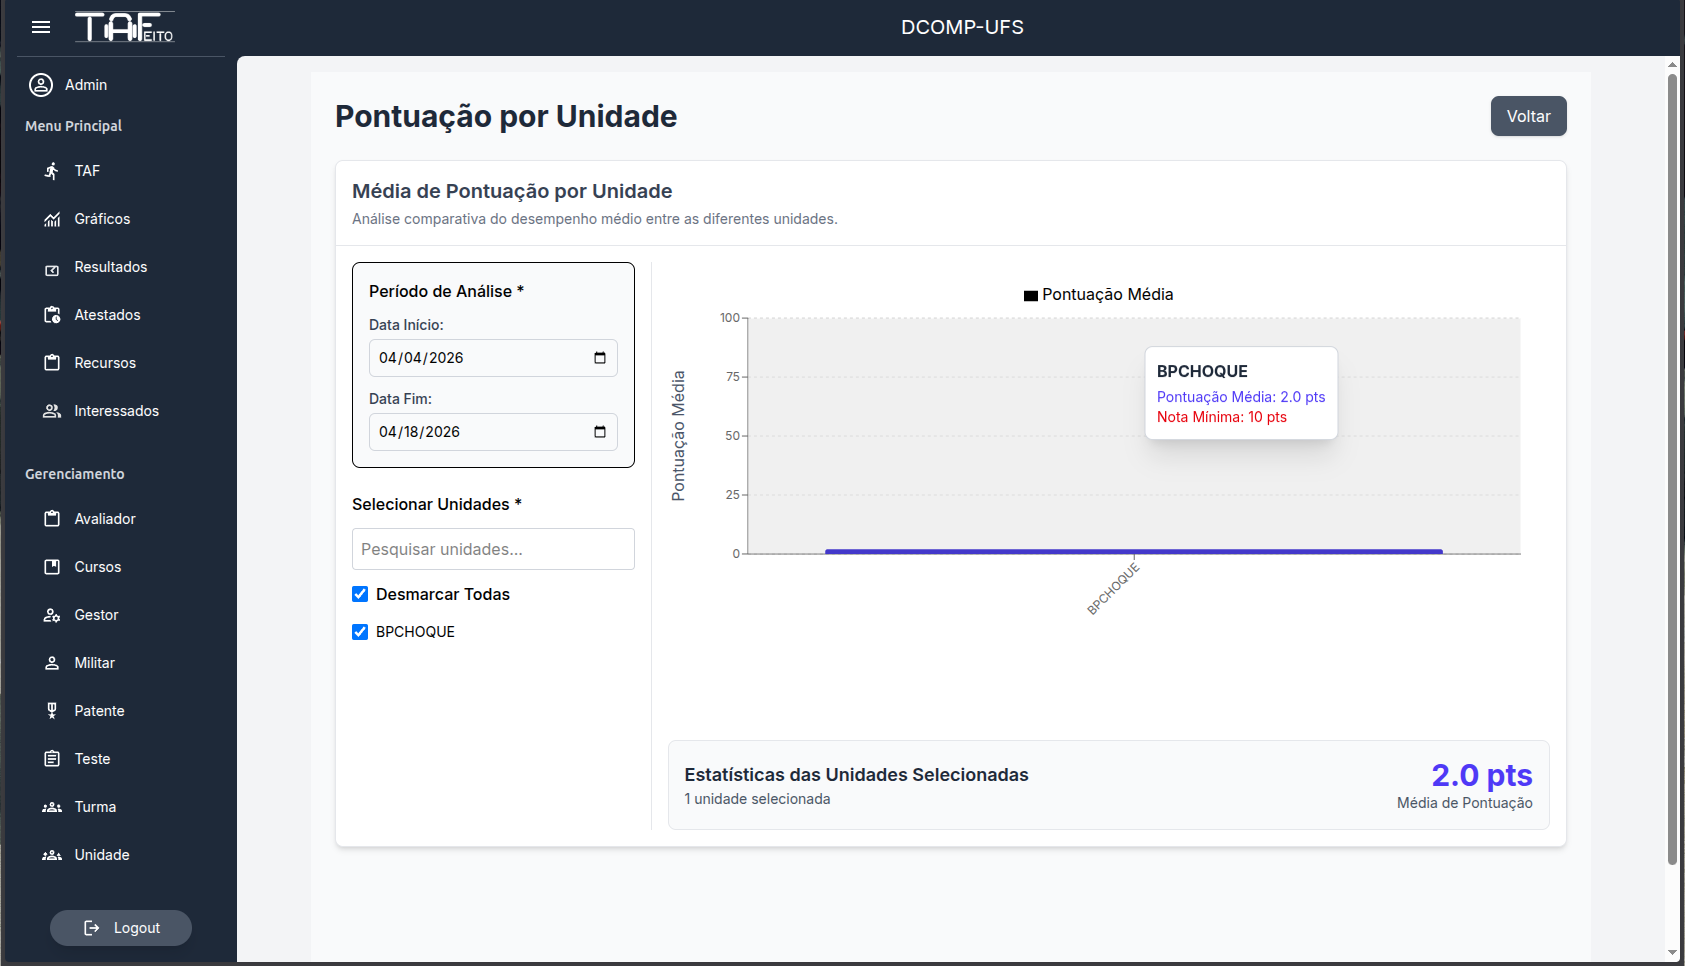
\includegraphics[scale=0.27]{./Imagens/tafeito/web/MediaPontuacaoUnidadeIngresso.png}
	\caption{Média de Pontuação por Unidade Ingresso}
	\label{fig:media_pontuacao_unidade_ingresso}
\end{figure}

\begin{itemize}
	\item \textbf{Evolução Temporal Unidade Periódico}: funcionalidade de gráfico vista por Coordenadores e Gestores cujo objetivo é mostrar a evolução dos resultados de TAFs aplicados a uma Unidade, ou seja, é possível identificar o desempenho da Unidade a partir dos TAFs que foram sendo aplicados ao longo do tempo, sendo exclusivo para TAFs periódicos (\autoref{fig:evolucao_temporal_periodico}). Também requer a seleção do período de aplicação do TAF e a Unidade para exibição dos dados.
\end{itemize}

\begin{figure}[H]
	\centering
	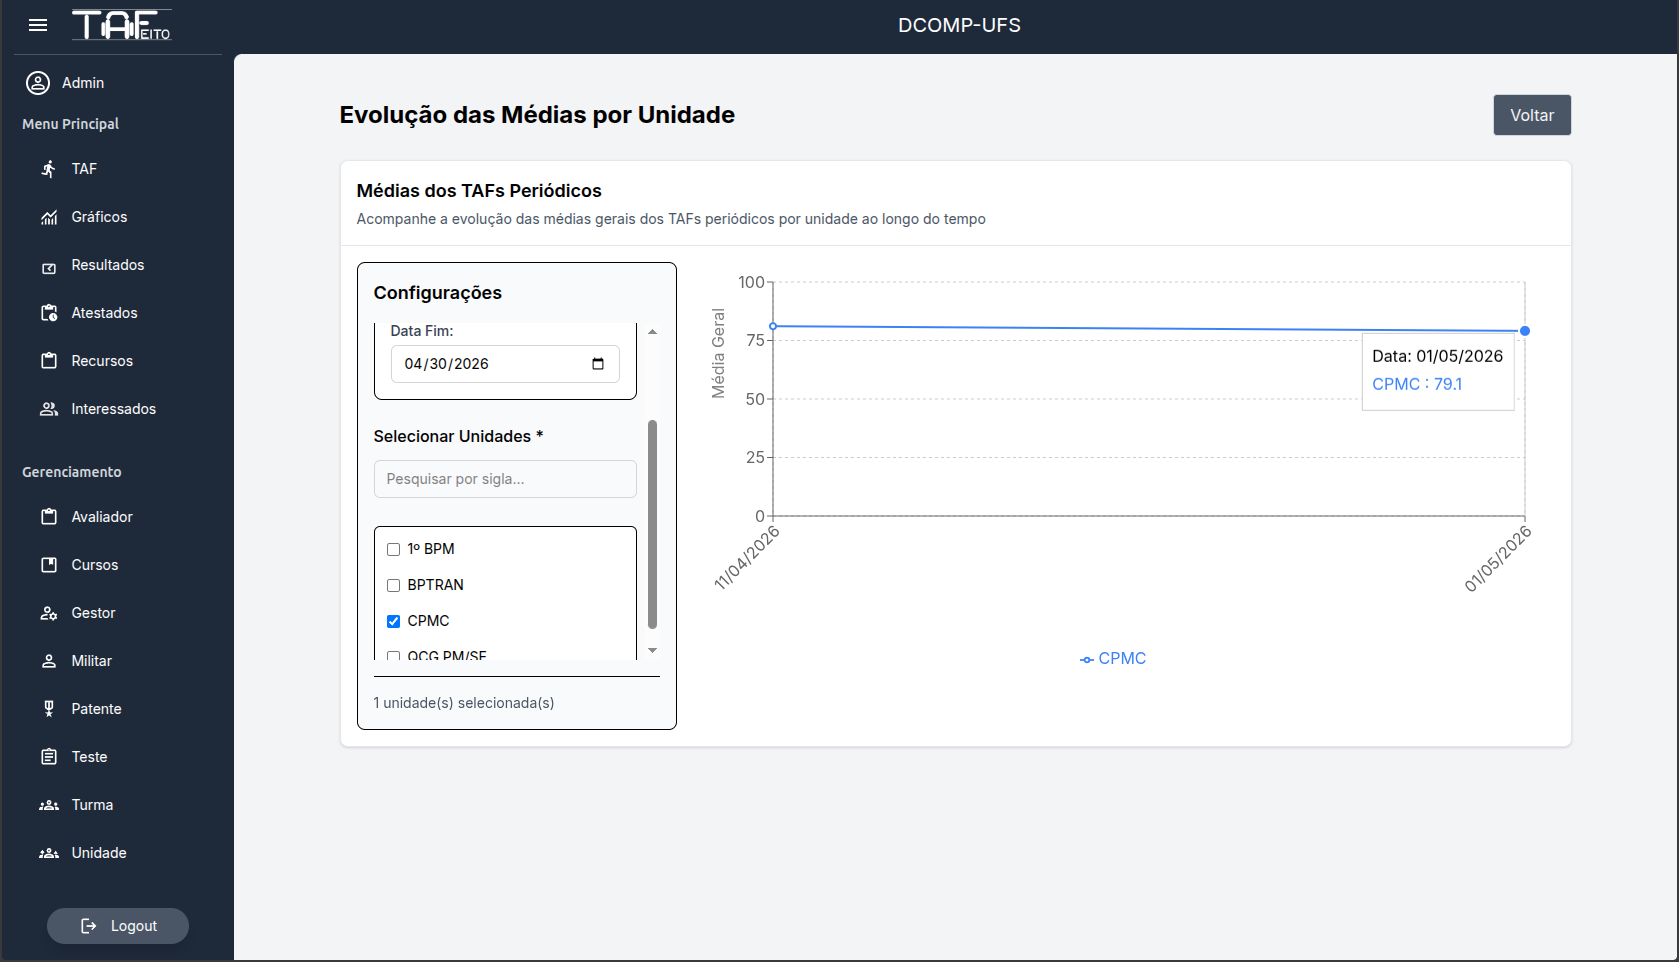
\includegraphics[scale=0.27]{./Imagens/tafeito/web/EvolucaoTemporalUnidadePeriodico.png}
	\caption{Evolução Temporal Unidade Periódico}
	\label{fig:evolucao_temporal_periodico}
\end{figure}

\begin{itemize}
	\item \textbf{Distribuição de Notas}: funcionalidade de gráfico vista por Coordenadores e Gestores cujo objetivo é mostrar a distribuição das notas de um TAF, sendo aplicados a Turmas ou Unidades (\autoref{fig:distribuicao_notas}). Nele, é possível verificar informações como a maior nota atingida, a Taxa de Aprovação, pontuações mais comuns, dentre outros (\autoref{fig:distribuicao_notas_taf}).
\end{itemize}

\begin{figure}[H]
	\centering
	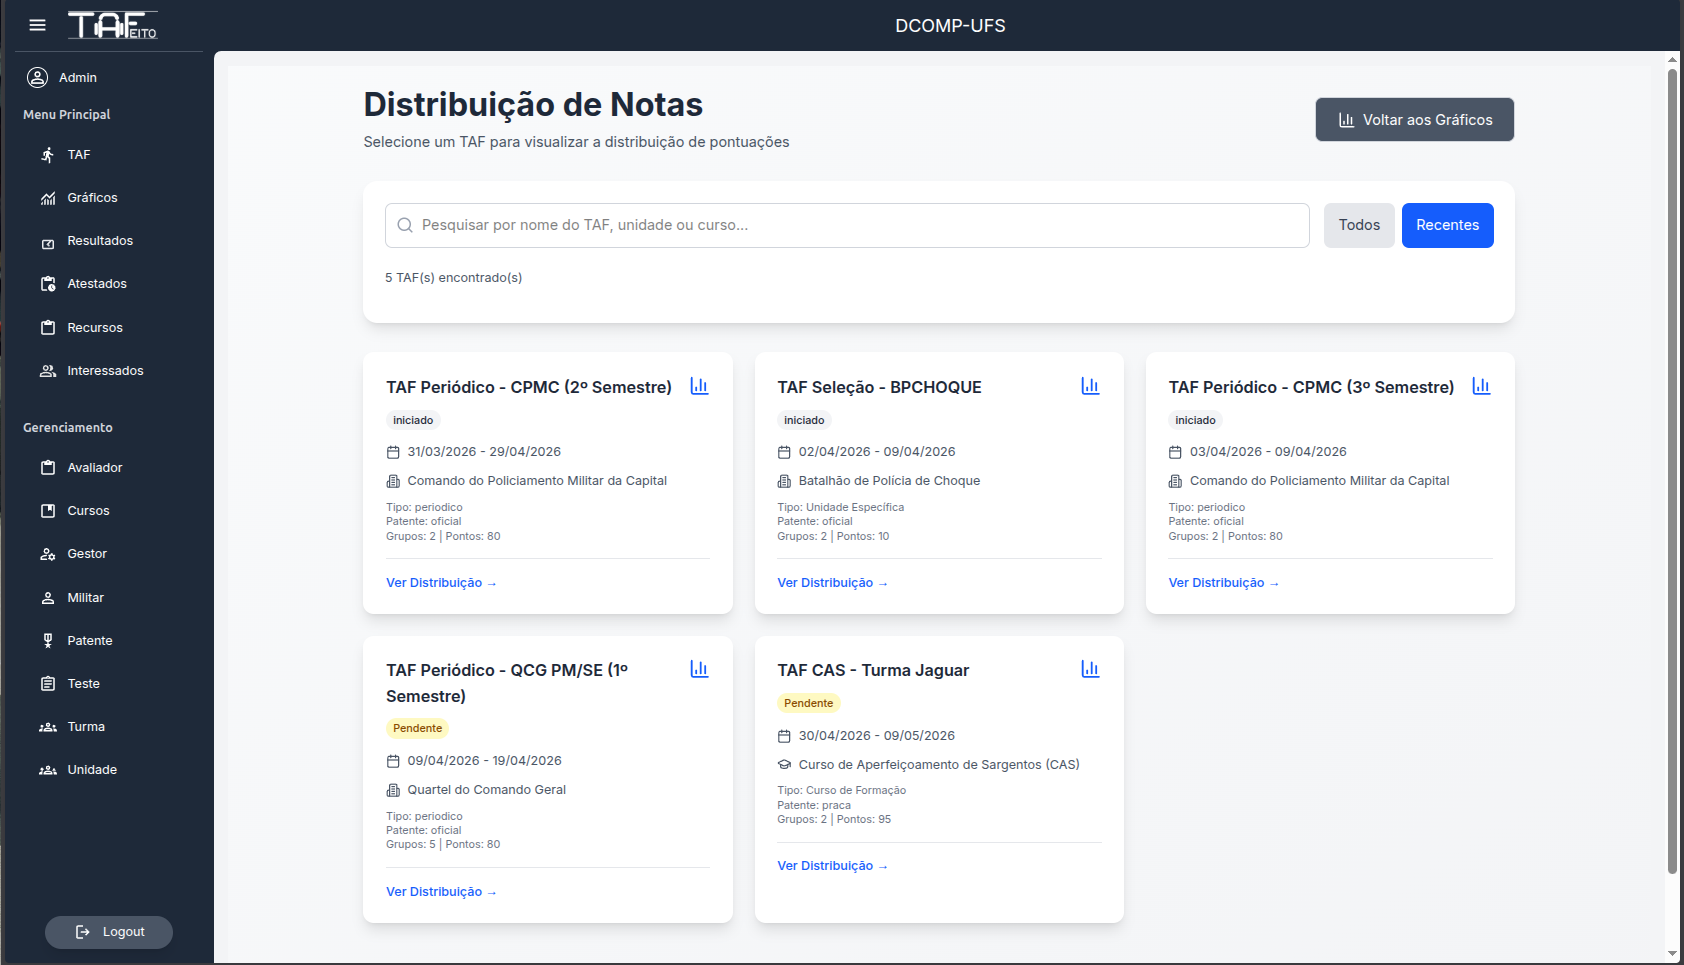
\includegraphics[scale=0.27]{./Imagens/tafeito/web/DistribuicaoNotasGeral.png}
	\caption{Distribuição de Notas}
	\label{fig:distribuicao_notas}
\end{figure}

\begin{figure}[H]
	\centering
	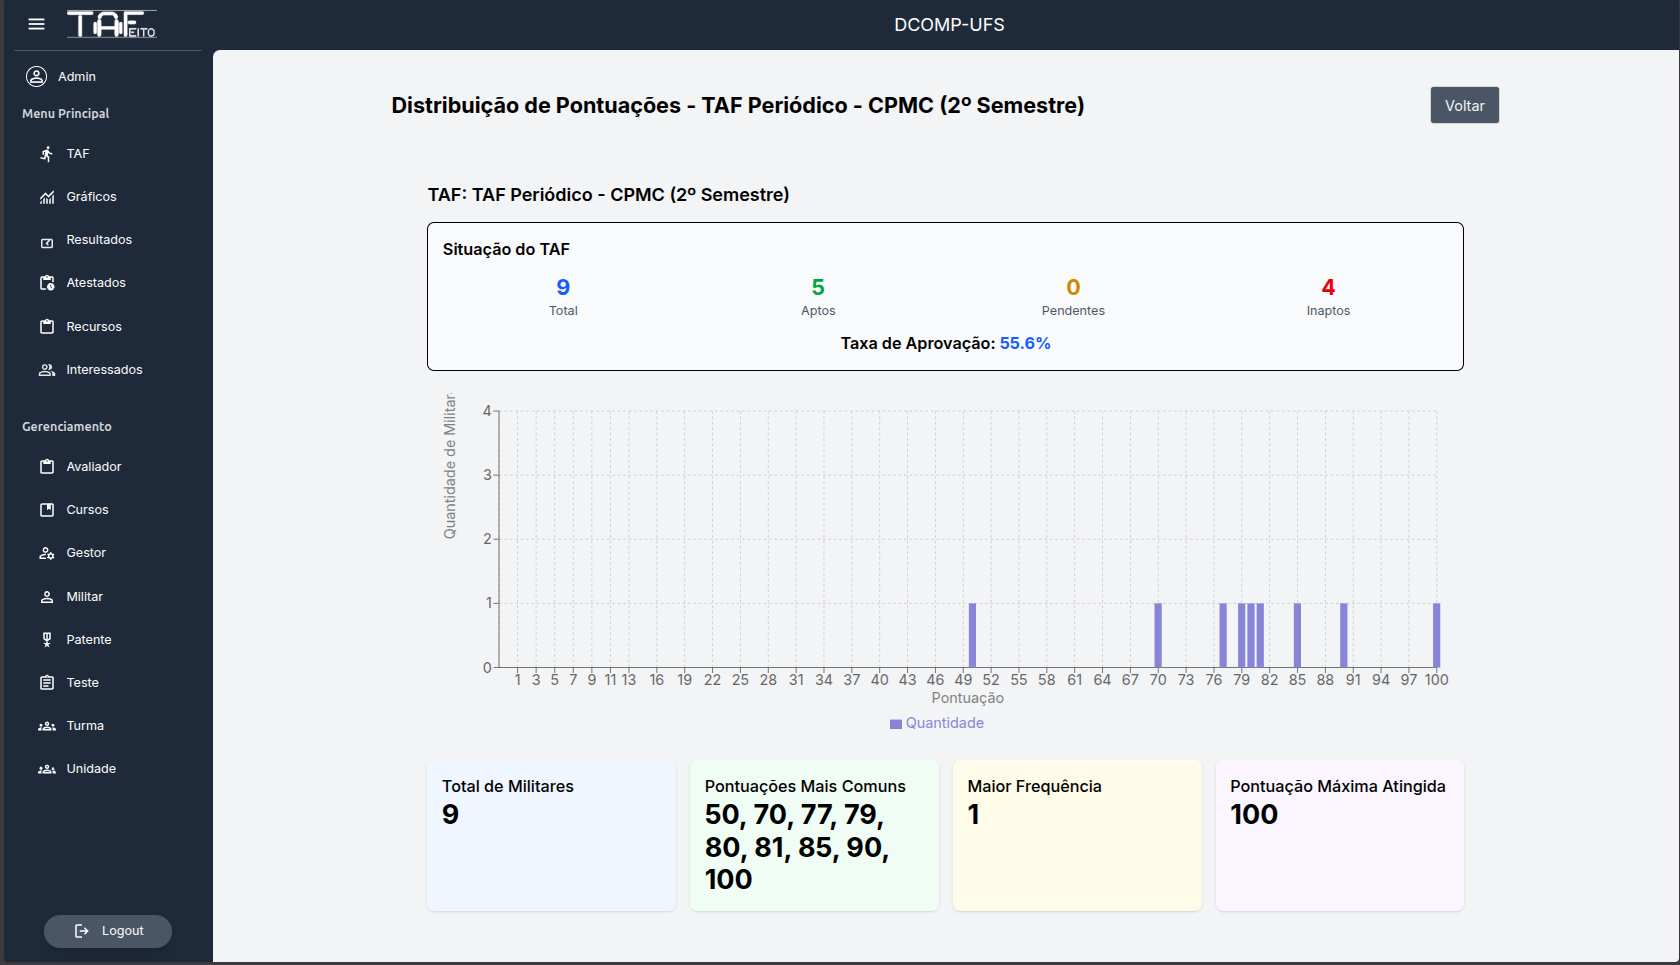
\includegraphics[scale=0.27]{./Imagens/tafeito/web/DistribuicaoNotasTaf.png}
	\caption{Distribuição de Notas para um TAF}
	\label{fig:distribuicao_notas_taf}
\end{figure}

\section{Funcionalidades da Versão Mobile}
A versão Mobile foi proposta com o intuito de poder executar o processo de avaliação da aptidão física dos integrantes das instituições militares, cumprindo as exigências estabelecidas pelo Coordenador no Portal Web (\ref{sec:funcionalidades_web}). As funcionalidades desta verssão serão explicitadas abaixo.

\begin{itemize}
	\item \textbf{Aplicar TAF}: funcionalidade executada apenas pelo Avaliador, é uma das principais funcionalidades presentes na versão \textit{Mobile}, sendo responsável pela execução dos testes definidos pelo Coordenador. Inicialmente, ao entrar com o perfil Avaliador, esta será a primeira funcionalidade a ser exibida, onde listarão todos os TAFs a serem executados ao qual o Avaliador faz parte (\autoref{fig:funcionalidade_aplicar_taf}), em seguida, deverá selecionar o Grupo, que é uma partição definida pelo Coordenador para facilitar a execução dos Testes por parte do Avaliador para uma quantidade menor de Militares sob sua responsabilidade (\autoref{fig:selecionar_grupo_taf}), em seguida, o Avaliador deverá selecionar o Exercício que aplicará a avaliação (\autoref{fig:selecionar_teste_taf}), selecionando os Militares (\autoref{fig:selecionar_militares}) e aplicar o Exercício, inserindo as métricas observadas (\autoref{fig:inserir_resultados}).
\end{itemize}

\begin{figure}[H]
	\centering
	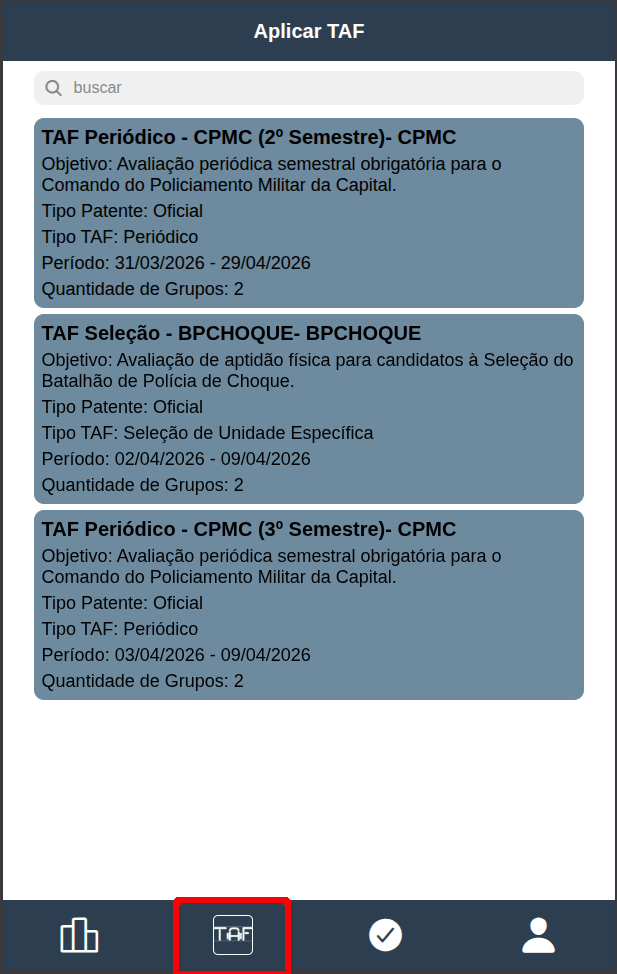
\includegraphics[scale=0.3]{./Imagens/tafeito/mobile/Aplicar_TAF.png}
	\caption{Funcionalidade Aplicar TAF}
	\label{fig:funcionalidade_aplicar_taf}
\end{figure}

\begin{figure}[H]
	\centering
	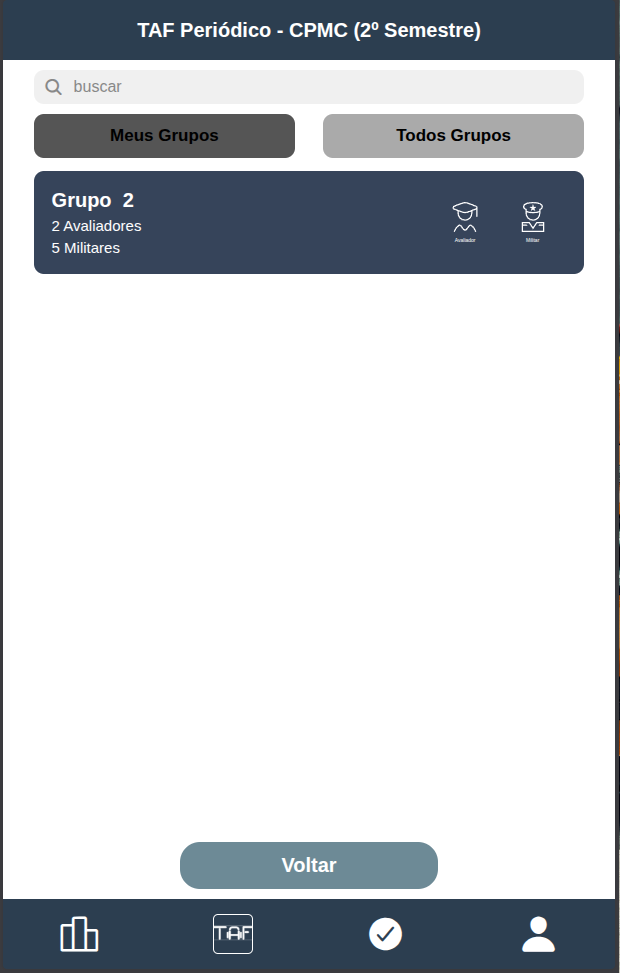
\includegraphics[scale=0.3]{./Imagens/tafeito/mobile/Selecao_Grupo_TAF.png}
	\caption{Selecionar Grupo do TAF}
	\label{fig:selecionar_grupo_taf}
\end{figure}

\begin{figure}[H]
	\centering
	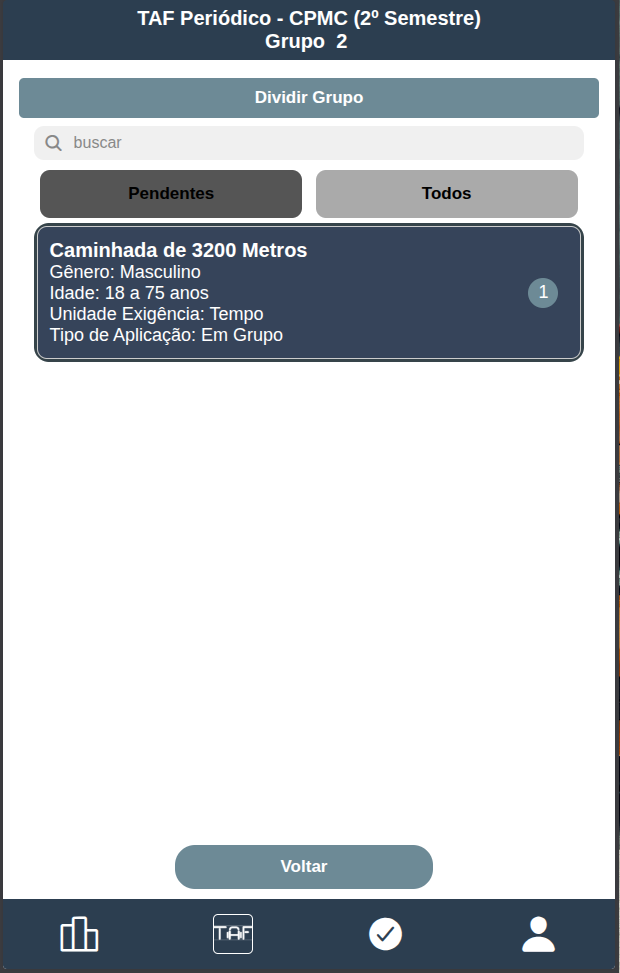
\includegraphics[scale=0.3]{./Imagens/tafeito/mobile/Selecao_Teste_TAF.png}
	\caption{Selecionar Teste do TAF}
	\label{fig:selecionar_teste_taf}
\end{figure}

\begin{figure}[H]
	\centering
	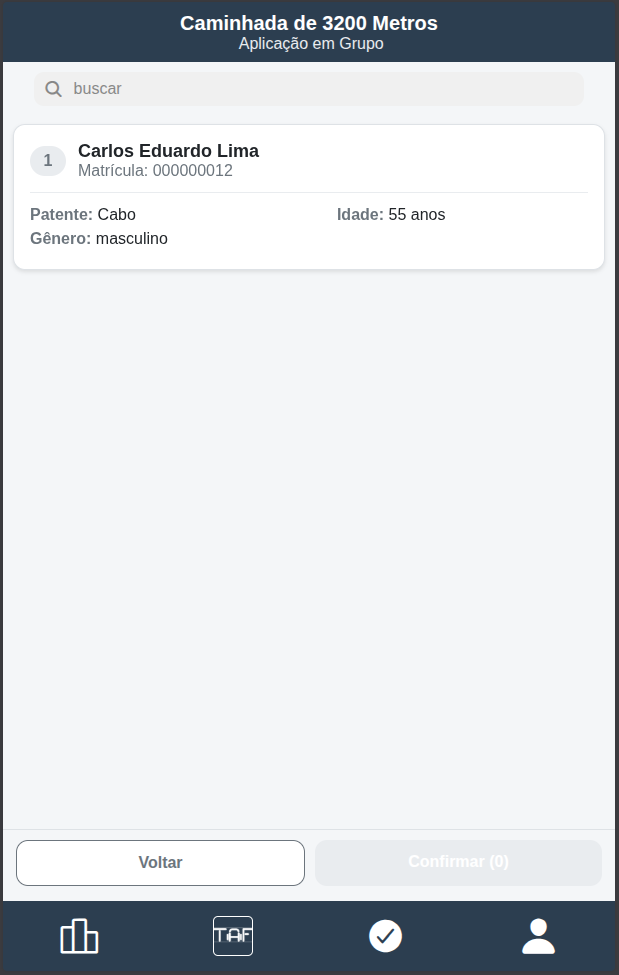
\includegraphics[scale=0.3]{./Imagens/tafeito/mobile/Selecao_Militar_TAF.png}
	\caption{Selecionar Militares do TAF}
	\label{fig:selecionar_militares}
\end{figure}

\begin{figure}[H]
	\centering
	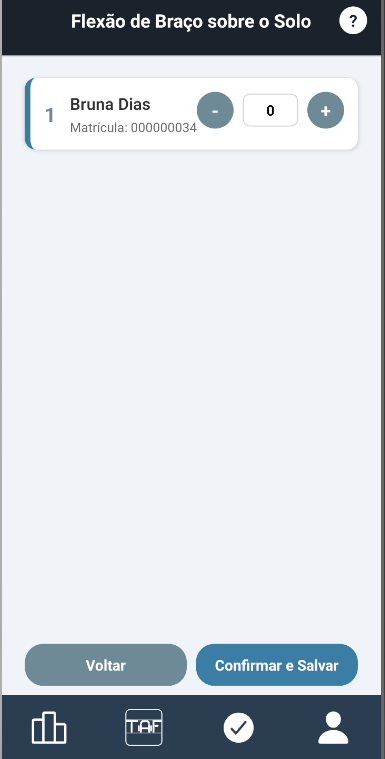
\includegraphics[scale=0.4]{./Imagens/tafeito/mobile/Insercao_Resultados_TAF.png}
	\caption{Inserir Resultado do Militar}
	\label{fig:inserir_resultados}
\end{figure}

\begin{itemize}
	\item \textbf{Autenticar Resultados do TAF}: funcionalidade executada apenas pelo Avaliador, é uma das principais funcionalidades presentes na versão \textit{Mobile}, devendo ser executada após a aplicação do TAF. Ela é responsável pela autenticação dos resultados obtidos pelos Militares. Inicialmente, o Avaliador deverá acessar a funcionalidade (\autoref{fig:funcionalidade_autenticar_resultados}) e seguir os mesmos passos da funcionalidade anterior até visualizar o resultado do Militar (\autoref{fig:confirmar_autenticacao}), onde deverá confirmar o resultado daquele Militar para o Exercício selecionado.
\end{itemize}

\begin{figure}[H]
	\centering
	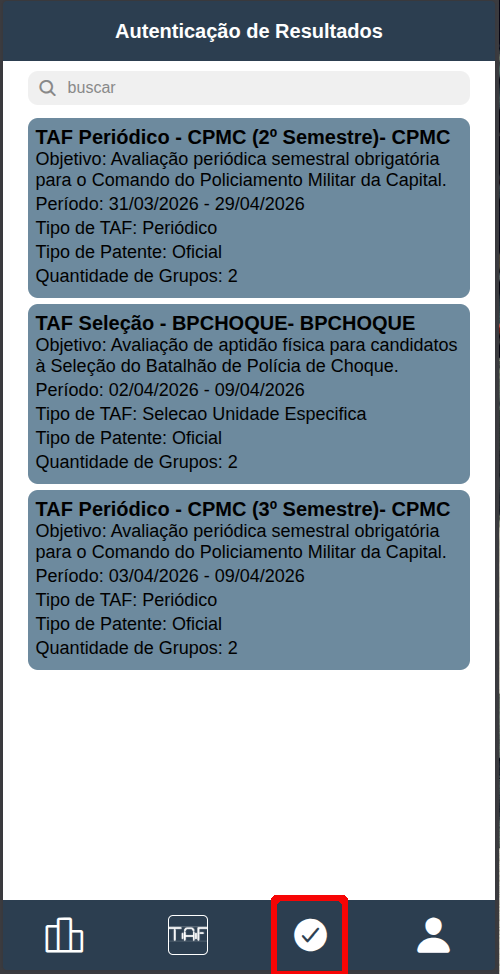
\includegraphics[scale=0.3]{./Imagens/tafeito/mobile/Autenticar_Resultados.png}
	\caption{Autenticar Resultados do TAF}
	\label{fig:funcionalidade_autenticar_resultados}
\end{figure}

\begin{figure}[H]
	\centering
	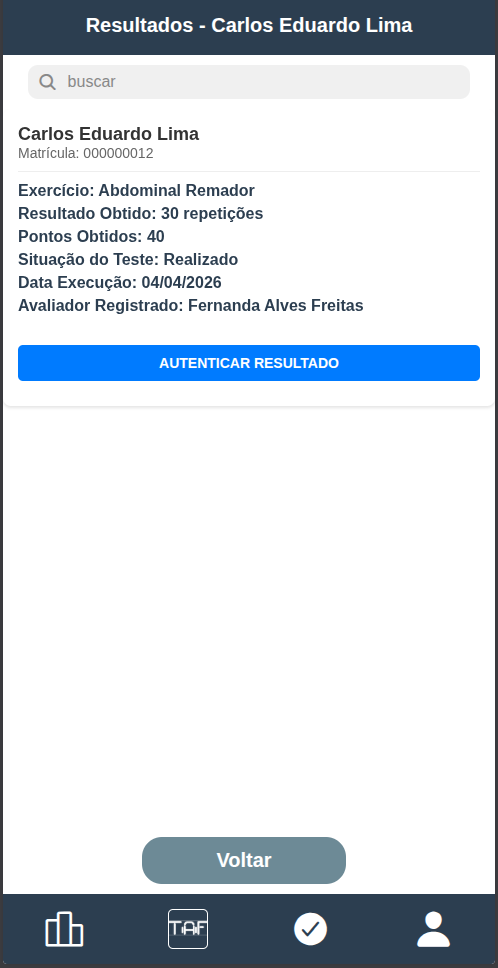
\includegraphics[scale=0.3]{./Imagens/tafeito/mobile/Confirmar_autenticacao.png}
	\caption{Confirmar Autenticação do Militar}
	\label{fig:confirmar_autenticacao}
\end{figure}

\begin{itemize}
	\item \textbf{Resultados do TAF}: funcionalidade executada pelo Avaliador e Militar. Ela é responsável pela visualização dos resultados obtidos pelos Militares, onde, para acessá-la, o Avaliador deverá seguir os mesmos passos da funcionalidade anterior até visualizar o resultado do Militar (\autoref{fig:confirmar_autenticacao}), onde poderá identificar quais exercícios foram concluídos e identificar sua porcentagem de conclusão. A diferença de visualização pelo Perfil Militar é que, ao selecionar um TAF já aparecerá seu resumo com mais informações como, por exemplo, pontuação máxima e mínima, além de poder entrar com Recurso em um exercício (\autoref{fig:resultados_perfil_militar}).
\end{itemize}

\begin{figure}[H]
	\centering
	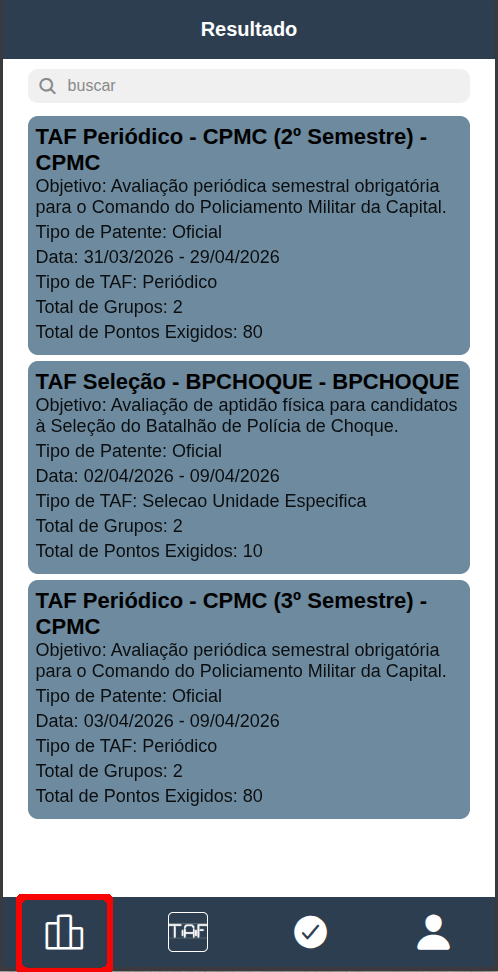
\includegraphics[scale=0.3]{./Imagens/tafeito/mobile/Resultados_TAF.png}
	\caption{Funcionalidade Resultados}
	\label{fig:funcionalidade_resultados}
\end{figure}

\begin{figure}[H]
	\centering
	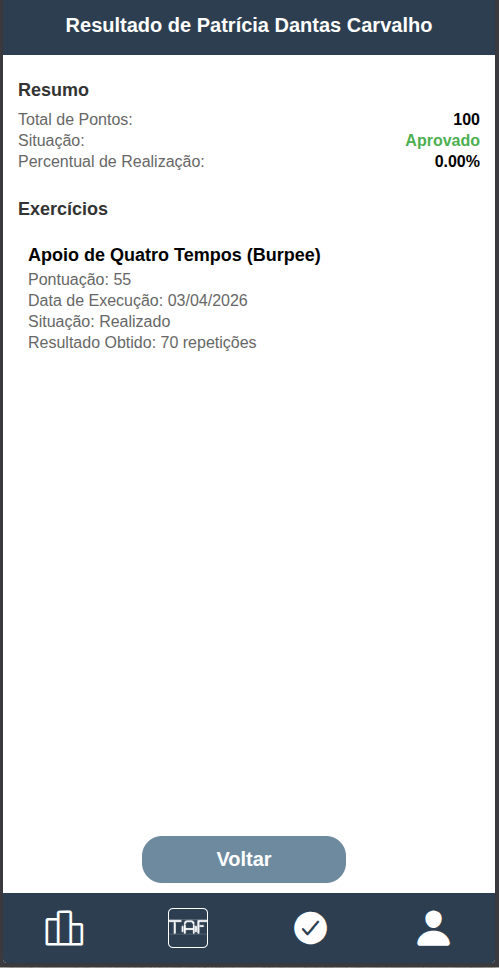
\includegraphics[scale=0.3]{./Imagens/tafeito/mobile/Resultado_Militar_TAF.png}
	\caption{Resultados do Militar no TAF}
	\label{fig:resultado_militar_taf}
\end{figure}

\begin{figure}[H]
	\centering
	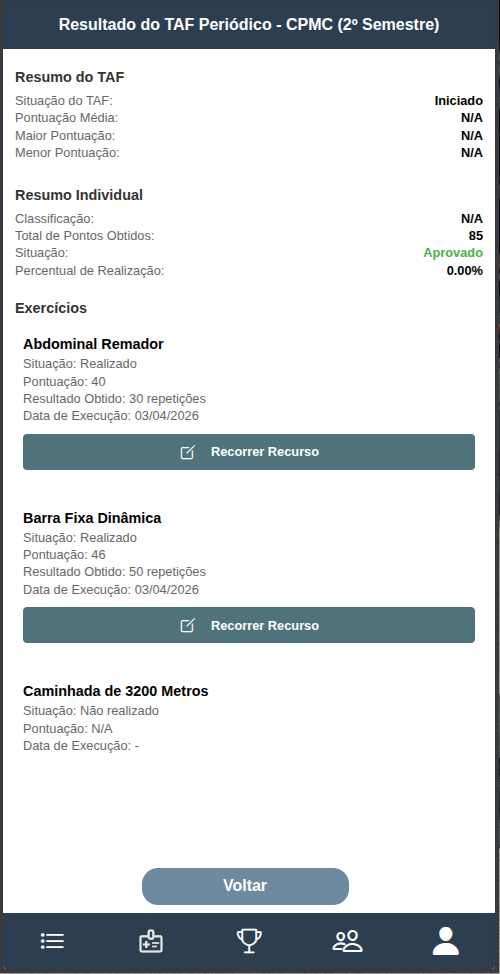
\includegraphics[scale=0.3]{./Imagens/tafeito/mobile/Resultados_Perfil_Militar.png}
	\caption{Resultados pelo Perfil Militar}
	\label{fig:resultados_perfil_militar}
\end{figure}

\begin{itemize}
	\item \textbf{Interesse no TAF}: funcionalidade executada apenas pelo Militar. Ela permitie que o Militar demonstre interesse em participar de um outro TAF ao qual ele não está incluso. Esses TAFs são direcionados para ingressar em uma nova Unidade, por isso há a necessidade de demonstração de interesse, por parte do Militar, para que o Coordenador, pela versão Web, possar autorizar ou não sua participação. O Militar apenas seleciona o TAF e confirma sua inscrição (\autoref{fig:interesse_no_taf}).
\end{itemize}

\begin{figure}[H]
	\centering
	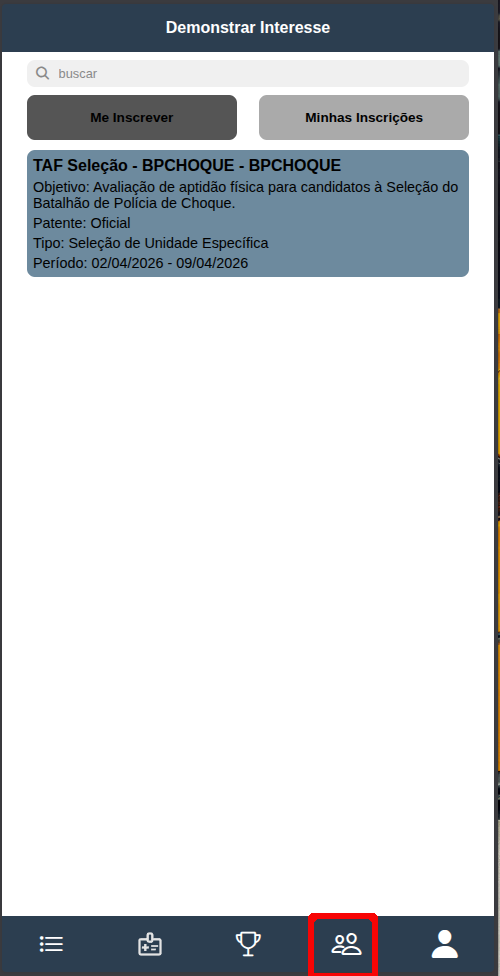
\includegraphics[scale=0.3]{./Imagens/tafeito/mobile/Interesse_TAF.png}
	\caption{Demonstrar Interesse no TAF}
	\label{fig:interesse_no_taf}
\end{figure}

\begin{itemize}
	\item \textbf{Atestado}: funcionalidade executada apenas pelo Militar. Ela permitie que o Militar adicione um atestado em um TAF, inserindo o motivo do não comparecimento e anexando um arquivo ou foto do atestado para análise do Coordenador (\autoref{fig:atestado_taf}).
\end{itemize}

\begin{figure}[H]
	\centering
	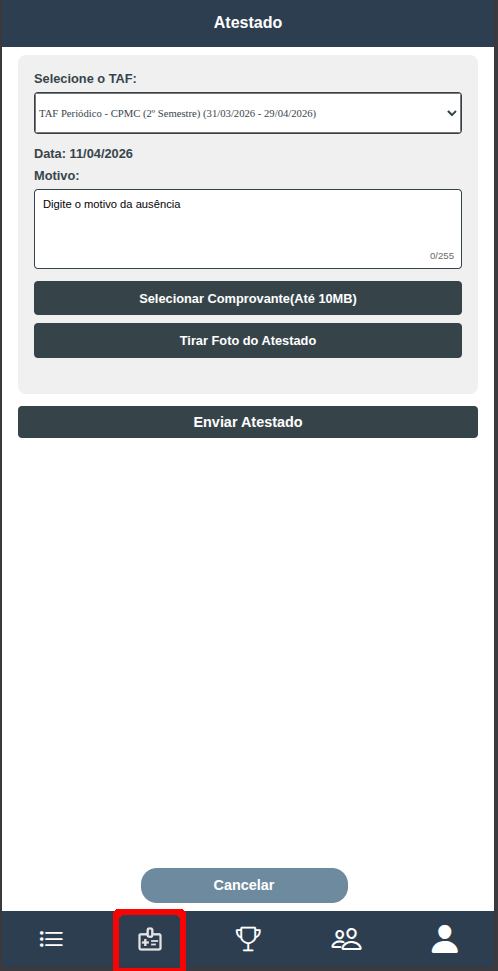
\includegraphics[scale=0.3]{./Imagens/tafeito/mobile/Atestado_TAF.png}
	\caption{Inserir Atestado no TAF}
	\label{fig:atestado_taf}
\end{figure}

\begin{itemize}
	\item \textbf{Ranking do TAF}: funcionalidade executada apenas pelo Militar. Ela permitie que o Militar visualize sua colocação e as dos demais integrantes naquele TAF, exibindo a pontuação total de cada um (\autoref{fig:ranking_taf}).
\end{itemize}

\begin{figure}[H]
	\centering
	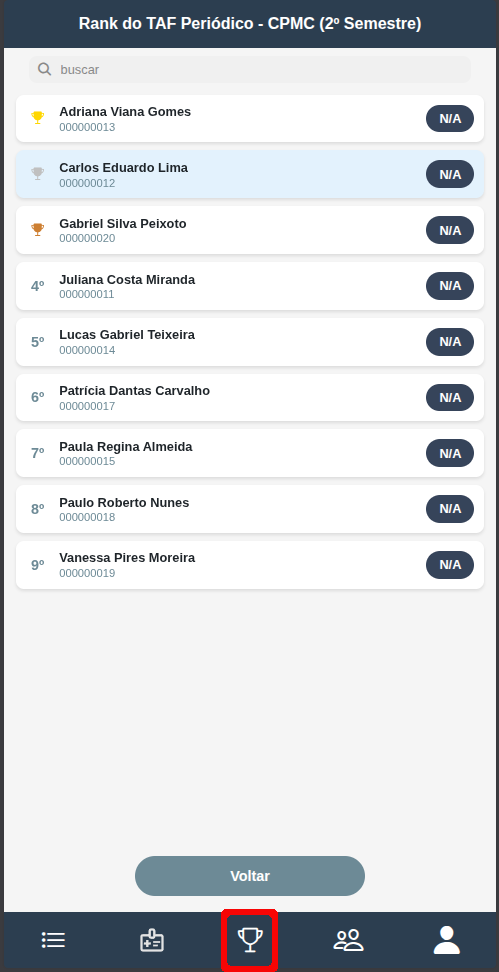
\includegraphics[scale=0.3]{./Imagens/tafeito/mobile/Ranking_TAF.png}
	\caption{Ranking do TAF}
	\label{fig:ranking_taf}
\end{figure}

\begin{itemize}
	\item \textbf{Perfil}: funcionalidade executada pelo Avaliador e Militar. Seu objetivo é mostrar ao usuário informações pessoais cadastradas e, caso seja acessado com o Perfil Avaliador, informações sobre os TAFs serão mostrados, como, por exemplo, o próximo TAF a ser aplicado, além de um botão para mudar entre os perfis (\autoref{fig:perfil_avaliador}). Já o perfil Militar será exibido apenas informações pessoais cadastradas, sendo possíveis alterá-las, além de um botão para mudança de senha, também disponíveis para o Perfil Avaliador (\autoref{fig:perfil_militar}).
\end{itemize}

\begin{figure}[H]
	\centering
	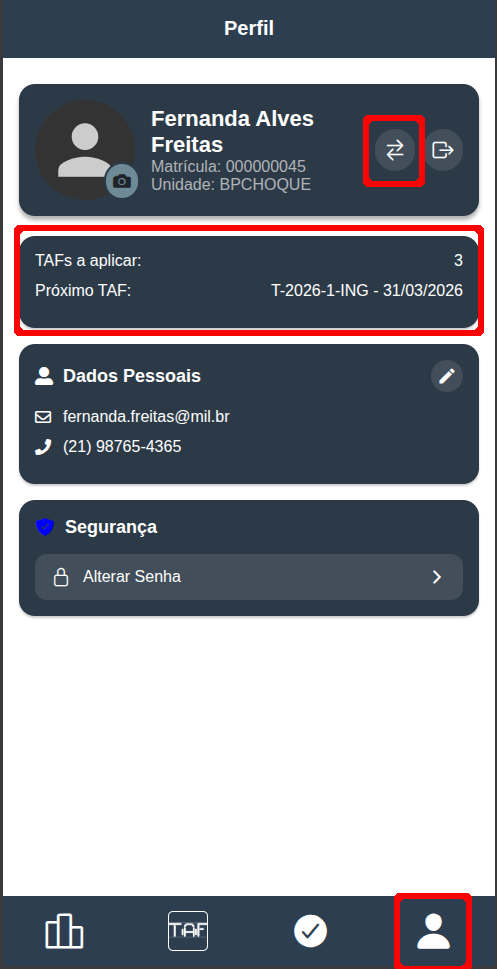
\includegraphics[scale=0.3]{./Imagens/tafeito/mobile/Perfil_Avaliador.png}
	\caption{Perfil Avaliador}
	\label{fig:perfil_avaliador}
\end{figure}

\begin{figure}[H]
	\centering
	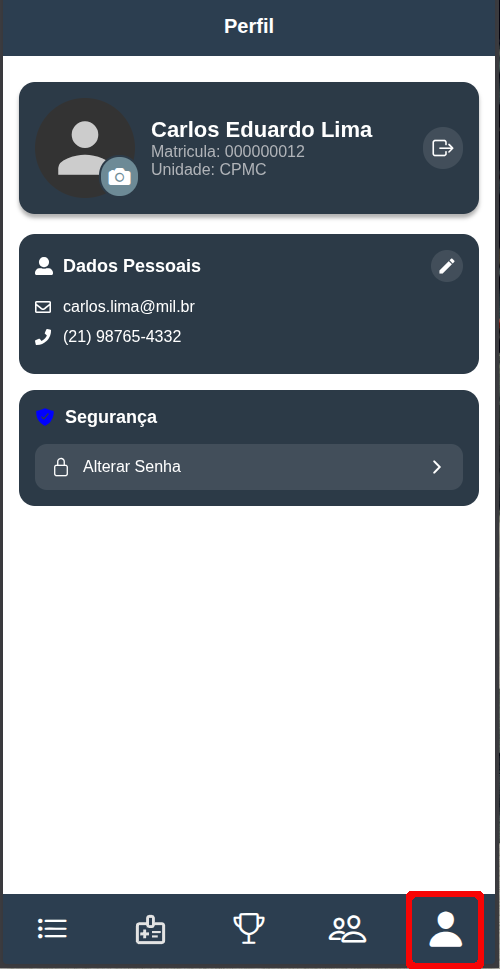
\includegraphics[scale=0.3]{./Imagens/tafeito/mobile/Perfil_Militar.png}
	\caption{Perfil Militar}
	\label{fig:perfil_militar}
\end{figure}

\section{Tecnologias Utilizadas}

Para atender as demandas do Projeto, o TAFeito possui uma ampla gama de tecnologias utilizadas para cada \textit{stack}, onde a linguagem selecionada para todo o Projeto foi a TypeScript, devido à sua tipagem. Para o \textit{Frontend} o \textit{framework} adotado foi o Next.js.\\ Já para o \textit{backend}, o \textit{framework} selecionado foi o NestJS,  direcionando todo o procedimento da API junto à criação da estrutura do Banco de Dados com as \textit{migrations} utilizando typeorm, ferramenta de ORM (Mapeamento Objeto-Relacional), o que possibilitou na agilidade de definições de tabelas e estruturas relacionais de cada entidade. Além disso, também há a presença da linguagem Python para manipulação de planilhas.\\ Para o \textit{mobile}, foi adotado o \textit{framework} React Native, onde possui semelhança com o \textit{frontend}, permitindo uma maior escalabilidade.\\ Com isso, foi finalizado o contexto do TAFeito após a matéria Prática Orientada em Computação (POC) II, mencionando tudo o que foi desenvolvido e os processos de dificuldades ultrapassadas durante toda a implementação, se fazendo necessário uma continuação e manutenção do Projeto para compor tudo que foi planejado no início da matéria POC I.

\chapter{TAFeito - Correções e Novas Funcionalidades}\label{novas_funcionalidades}

Este capítulo possui como objetivo apresentar o resultado obtido após a execução deste trabalho, assim como as dificuldades e alterações que foram necessárias após a execução dos testes exploratórios. Primeiramente, serão apresentadas as pendências existetes após a matéria POC II, seguindo, logo após, por uma explicação e demonstração das novas funcionalidades desenvolvidas. Por fim, serão elucidados os desafios obtidos após a execução dos testes exploratórios.

\section{Correções Necessárias}

Durante as execuções das atividades de POC II, algumas pendências foram deixadas após a execução dos testes exploratórios, pois, devido ao prazo dessa matéria, não foi possível atender todas as demandas. Sendo assim, parte delas foram vislumbradas para a execução deste trabalho, como podem ser verificadas no \autoref{quad:pendencias_poc_ii}.

\begin{quadro}[H]
    \caption{Pendências de POC II \label{quad:pendencias_poc_ii}}
    \centering
    \begin{tabular}{|>{\raggedright\arraybackslash}p{4cm}|
                >{\raggedright\arraybackslash}p{4cm}|
                >{\raggedright\arraybackslash}p{2cm}|
                >{\raggedright\arraybackslash}p{2cm}|}
        \hline
        Funcionalidade & Descrição & Ator & Modalidade \\
        \hline
        Desabilitar Perfil Gestor na Remoção da Unidade & Permanência do perfil Gestor após exclusão de uma Unidade & Gestor & \textit{Web} \\
        \hline
        Exclusão de uma Unidade com Militar(es) associado(s) & Exclusão de uma Unidade com Militar(es) associado(s) &Coordenador & \textit{Web} \\
        \hline
        Cadastro de Unidade com um Comandante de outra Unidade & Permissão de cadastro de um outro Comandante na criação de uma nova Unidade & Coordenador & \textit{Web} \\
        \hline
        Transferência de Militar para outra Turma & Padronização da funcionalidade de transferência de Militar(es) entre Turmas e Unidades & Coordenador & \textit{Web} \\
        \hline
        Auditoria & Capturar todas as transações de dados feitos na Aplicação & Coordenador & \textit{Web} \\
        \hline
        Ajustar Inserção de Avaliadores em um TAF & Inserção de Avaliadores nos subgrupos dos grupos já existentes em um TAF & Coordenador & \textit{Web} \\
        \hline
        Adicionar Militares por CSV & Adição de Militares por arquivos CSV & Coordenador & \textit{Web} \\
        \hline
        Execução em Tempo Real & Compartilhamento dos resultados dos Militares em tempo real entre os Avaliadores nos testes & Avaliador & \textit{Mobile} \\
        \hline
        Remoção de Curso atrelado à Turma & Exibição de erro não tratado do Banco de Dados ao remover um Curso com uma Turma atrelada & Coordenador & \textit{Web} \\
        \hline
        Edição do nome da Unidade & A edição do nome da Unidade ocasionava em um erro não tratado pelo Backend & Coordenador & \textit{Web} \\
        \hline
        Visualização de TAF pelo Avaliador & Avaliador visualiza os TAFs, mas não visualiza os Grupos dos mesmos & Avaliador & \textit{Web} \\
        \hline
        Visualizações dos TAFs pelos Perfis Gestor, Coordenador e Avaliador & Os perfis citados conseguem visualizar TAFs aos quais não possuem relações diretas & Gestor, Coordenador e Avaliador & \textit{Web} \\
        \hline
    \end{tabular}
\end{quadro}

\section{Novas Funcionalidades}

Para este trabalho foram houve uma preocupação em solucionar as pendências listadas anteriormente.

\subsection{Desabilitar Perfil Gestor na Remoção da Unidade}
\label{sub:desabilitar_gestor_remocao_unidade}

No contexto do TAFeito, o Gestor é aquele Militar responsável por uma Unidade, ou seja, ele visualiza, no sistema, todas as informações voltadas para aquela Unidade, desde os TAFs aplicados até os Atestados, Recursos, desempenho dos Militares, etc. Isso permite um controle visual tático de possíveis ações que podem ser tomadas com seus subordinados. Seria extritamente antiético e nada constitucional permitir que um Gestor destituído do seu papel ainda visualize as informações presentes no sistema que condizem com a Unidade ao qual ele já fez parte, por isso se faz necesssário a remoção desse perfil ao Militar comandante da Unidade, caso esta seja removida.

Este problema se trata de um \textit{bug} de regra de negócio não tratado. Onde, como já explicado anteriormente, consiste em manter o perfil de Gestor ao Militar após uma Unidade ser removida, trazendo uma quebra na regra de negócio, pois permite que o Militar visualize informações que não mais lhe competem. Por isso, a forma de converter este problema foi remover, durante o processo de remoção da Unidade, o perfil de Gestor do Militar que comanda esta Unidade, como pode ser visto na \autoref{fig:remocao_perfil_gestor_exclusao_unidade}.

\begin{figure}[H]
	\centering
	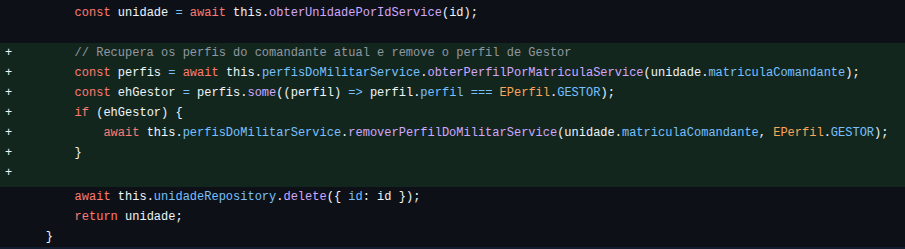
\includegraphics[scale=0.65]{./Imagens/tafeito/api/remocao_perfil_gestor.png}
	\caption{Remoção Perfil Gestor ao Excluir Unidade}
	\label{fig:remocao_perfil_gestor_exclusao_unidade}
\end{figure}

Portanto, após uma Unidade ser removida, não haverá mais o Comandante, pois perderá o perfil de Gestor e o Militar que possuía este papel não visualizará dados referente à esta Unidade.

\subsection{Exclusão de Unidade com Militar(es) Associado(s)}
\label{sub:exclusao_unidade_lotacao_militar}

Além de um Gestor, uma Unidade possui Militares integrantes nela por meio de Lotações, ou seja, significa que o Militar está lotado em uma Unidade. Essa lotação possui um período, referente ao tempo presente do Militar à Unidade, portanto, não pode haver uma Lotação sem uma Unidade existente. Na modelagem do Banco de Dados, esta restrição está explícita e a operação é bloqueada caso haja uma remoção de um registro de Unidade com Lotações associadas, mas o erro é repassado ao usuário final, causando grandes problemas de UX/UI, pois traz confusão a respeito do que poderia ter levado àquele erro.

O \textit{bug} refere-se à uma violação na regra de negócio onde há uma remoção da Unidade com Lotações de Militares associadas, não devendo ser permitido esta ação, pois, para que uma Lotação exista, é obrigatória a presença de uma Unidade. A fim de solucionar este problema foi necessário importar o Módulo de \textit{Service} da Lotação e realizar verificações das Lotações existentes para aquela Unidade, lançando um erro tratado ao usuário, como pode ser visto na \autoref{fig:remocao_unidade_com_lotacao}.

\begin{figure}[H]
	\centering
	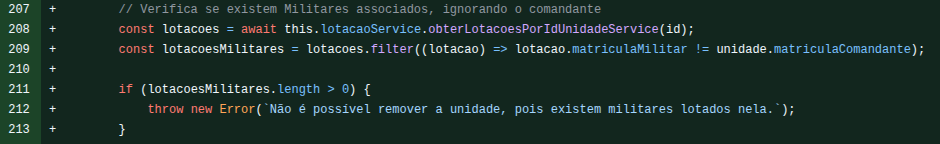
\includegraphics[scale=0.63]{./Imagens/tafeito/api/remocao_unidade_lotacao.png}
	\caption{Remoção Unidade com Militares Lotados}
	\label{fig:remocao_unidade_com_lotacao}
\end{figure}

Portanto, há uma transparência ao usuário do que se trata a mensagem de erro presente na tela, conferindo significado real da consequência da ação tomada por ele.

\subsection{Cadastro de Unidade com Comandante de outra Unidade}
\label{sub:cadastro_unidade_comandante_outra_unidade}

Como explicado na \autoref{sub:desabilitar_gestor_remocao_unidade}, o Gestor é o papel desempenhado pelo Comandante da Unidade. Como cada uma possui um papel/função diferente das demais, há a necessidade de dedicação exclusiva de um único Militar para gerenciar cada área, ou seja, no TAFeito, cada Militar Comandante deve estar associado a apenas uma única Unidade. Com isso, inserir um mesmo Comandante em mais de uma Unidade cria uma sobrecarga de funções, devendo ser barrada esta ação no sistema. A atribuição é feita durante o cadastro da Unidade, por isso, na opção de seleção, deve-se ocultar os Militares que já possuem algum tipo de associação de nível Comandante em alguma outra Unidade. Pensando nisso, foi reajustado o método responsável pela criação de Unidades, verificando se o Militar Comandante passado pela requisição já possui algum outro vínculo, como mostrado na \autoref{fig:cadastro_unidade_comandante_outra_unidade}.

\begin{figure}[H]
	\centering
	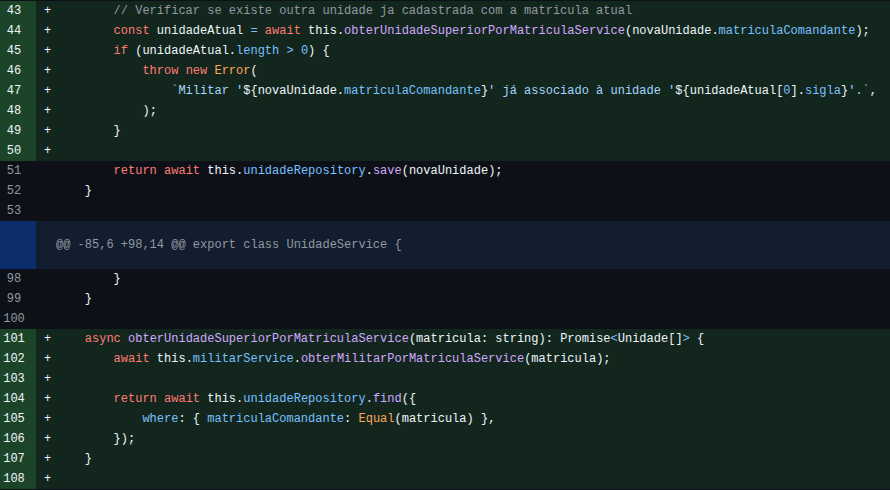
\includegraphics[scale=0.6]{./Imagens/tafeito/api/cadastro_comandante_outra_unidade.png}
	\caption{Cadastro de Unidade com Comandante de outra Unidade}
	\label{fig:cadastro_unidade_comandante_outra_unidade}
\end{figure}

O método \textit{obterUnidadeSuperiorPorMatriculaService} obtém todas as unidades que possuem a Matrícula do Comandante igual à matrícula fornecida, acusando um erro tratado a respeito da existência de tal Militar. Já na funcionalidade exibida ao usuário (\autoref{fig:unidades}), só será listado todos os Militares de nível oficial que não possuem nenhum relacionamento com outras Unidades.

\subsection{Transferência de Militar entre Turmas}

A Turma é outra forma de poder agrupar os Militares para aplicação do TAF. O Coordenador possui a liberdade para manipular os Militares existentes nas Turmas, desde que não possua um TAF associado à ela e, caso possua, ele ainda deve estar com \textit{status} pendente. Esta funcionalidade também está presente na página da listagem de Militares, porém apenas para uma transferência de Unidade e também há a transferência de Turma, porém o usuário deveria acessar a edição do Militar para realizar esta ação, o que traria bastante confusão e falta de padronização. Pensando da perspectiva de UX/UI, esta disposição de funcionalidades não deveria acontecer, pois induz ao erro, além de trazer uma complexidade à mais na utilização da ferramenta. Por isso, optou-se por dispor a funcionalidade de troca de Turma para o mesmo local onde já havia a troca de Unidade, como pode ser observado pela \autoref{fig:troca_de_turma}.

\begin{figure}[H]
	\centering
	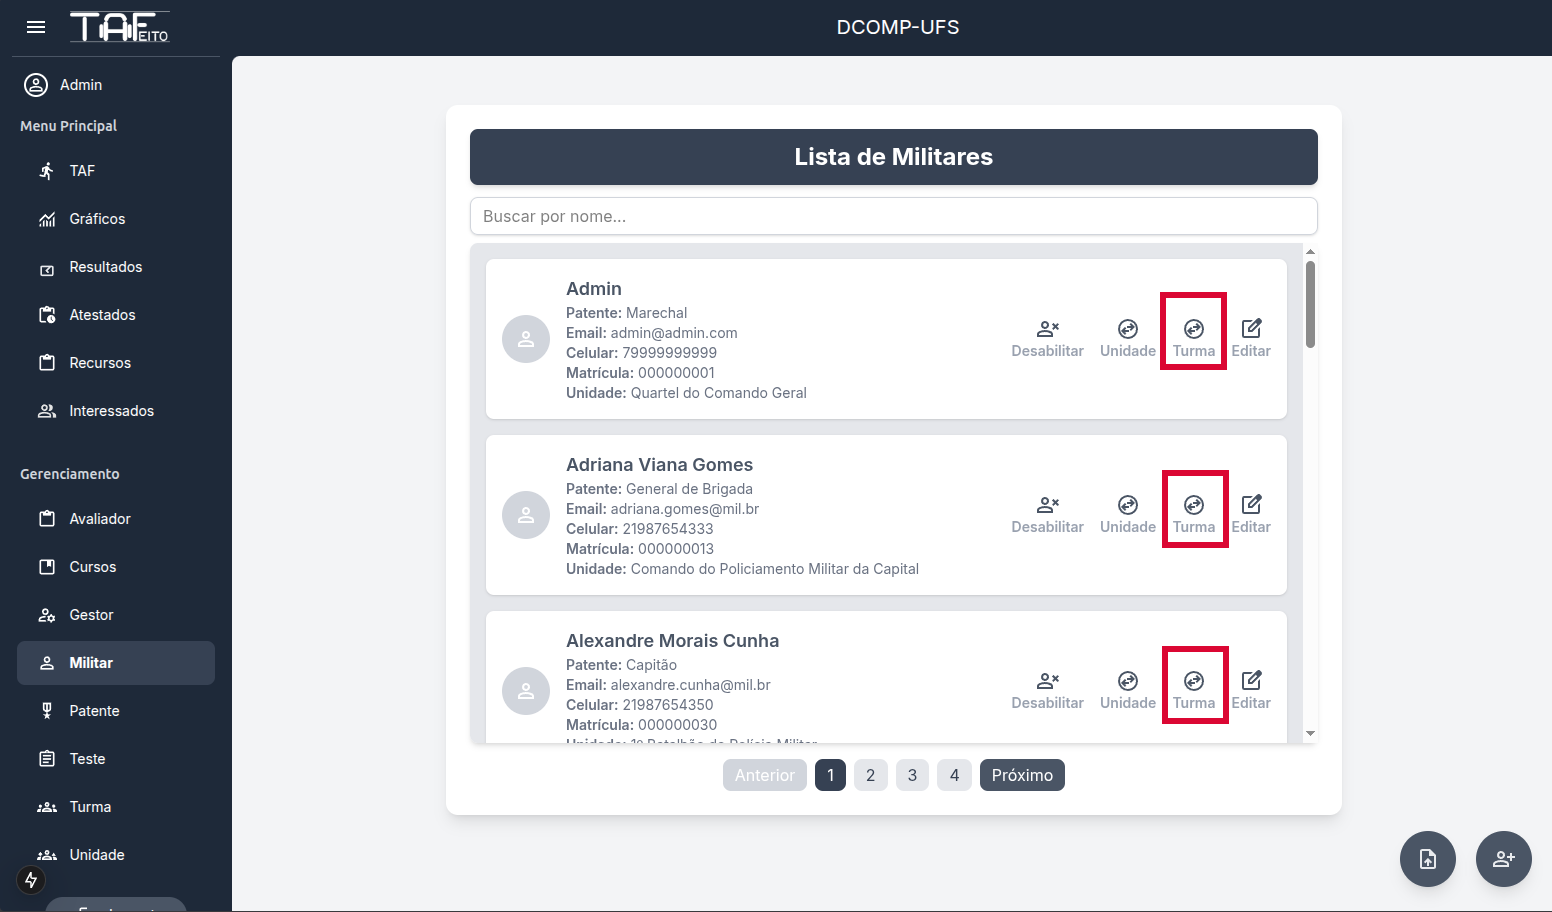
\includegraphics[scale=0.3]{./Imagens/tafeito/api/troca_de_turma.png}
	\caption{Funcionalidade Troca de Turma}
	\label{fig:troca_de_turma}
\end{figure}

\subsection{Auditoria}
\subsection{Inserção de Avaliador em um TAF}

Para garantir que os Avaliadores não se sobrecarreguem com as avaliações dos Militares, foi estebelecido o conceito de Grupos, onde são criados conforme a decisão do Coordenador na criação do TAF. Esses Grupos consistem em separar, a princípio, de forma igualitária, os Militares a serem avaliados, cabendo ao Coordenador decidir qual Avaliador ficará responsável pelo Grupo. Assim como existem os Subgrupos, que são criados para quando a quantidade de Militares presentes no Grupo excedem a capacidade do Avaliador, porém, este somente é criado pelos próprios Avaliadores antes da aplicação do TAF. O Coordenador poderá remanejar, de forma ilimitada, as disposições desses Avaliadores e a quantidade de Grupos, desde que o TAF não tenha iniciado. A API desenvolvida trata da estrutura necessária para realizar essa composição, desde o processo para redefinição da quantidade de Grupos presentes nos TAFs até a inserção ou remoção de Militares ou Avaliadores, porém, quando há a presença de Subgrupos, torna-se difícil realizar esta disposição, pois seria necessário uma verificação, de forma recursiva, a composição de cada Grupo e Subgrupos presentes.

Em uma versão anterior à desenvolvida neste trabalho, a remoção de um Avaliador de um TAF também o retirava dos Subgrupos, porém, para a adição de um Avaliador em um TAF com a estrutura de Grupos e Subgrupos já formada, não era feito essa redistribuição nos Subgrupos, apenas no Grupo Pai diretamente inserido. Por isso, este \textit{bug} foi classificado como de alta dificuldade devido à lógica necessária para adequar a inserção desses novos Avaliadores na estrutura dos Grupos já existentes. Foi identificado que este problema ocorria tanto na edição da quantidade de Grupos, quanto na inserção de Avaliadores em um TAF, já que estavam relacionados com a redefinição de Grupos presentes.

Com efeito, alguns métodos precisaram ser adicionados para solucionar o problema mencionado. Dentre eles, era necessário percorrer a estrutura hierárqica dos Grupos e armazenar quais os subgrupos existentes, por isso, foi desenvolvido o método existente na \autoref{fig:obter_estrutura_grupo}.

\begin{figure}[H]
	\centering
	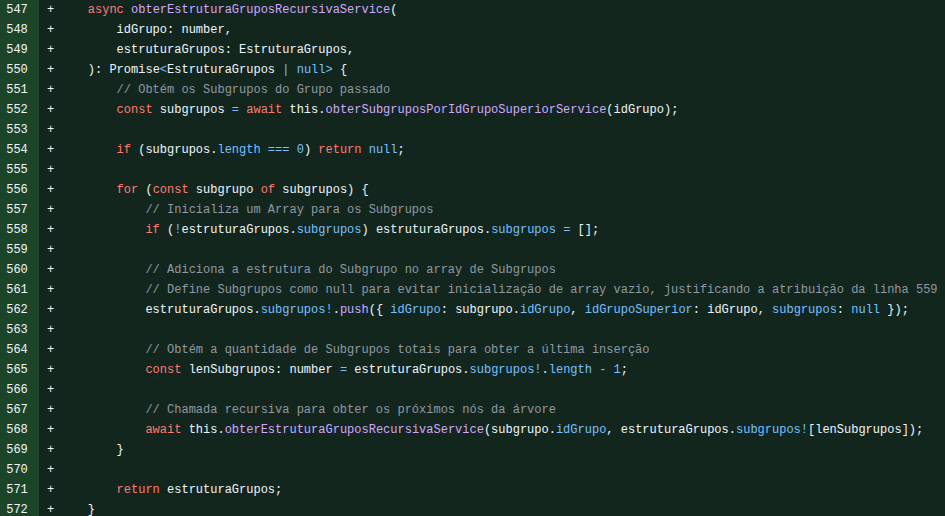
\includegraphics[scale=0.6]{./Imagens/tafeito/api/obter_estrutura_grupos.png}
	\caption{Método para obter a estrutura de um Grupo}
	\label{fig:obter_estrutura_grupo}
\end{figure}

Este método permite passar como parâmetro o ID de um Grupo, podendo ser um Grupo raiz ou um Grupo filho, e retornar sua estrutura até o Grupo folha, sendo fundamental para evitar complexidade adicional aos demais métodos.

Um outro método essencial à execução trata da inserção do Avaliador no Grupo passado por parâmetro, realizando verificações para saber se ele já está inserido nos Subgrupos desse mesmo Grupo, como mostra a \autoref{fig:verifica_insere_avaliador_grupo}.

\begin{figure}[H]
	\centering
	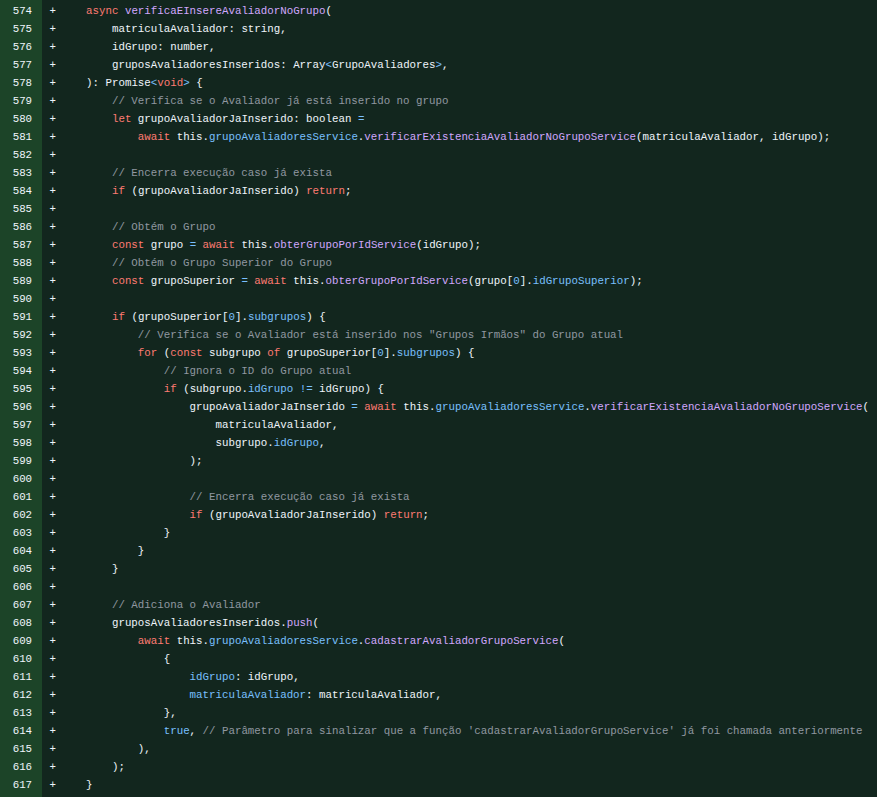
\includegraphics[scale=0.6]{./Imagens/tafeito/api/verificar_avaliador_grupo.png}
	\caption{Método para verificar e inserir Avaliador no Grupo}
	\label{fig:verifica_insere_avaliador_grupo}
\end{figure}

Por fim, há um método que centraliza e comanda as inserções dos Avaliadores nos Subgrupos, como ilustrado na \autoref{fig:insere_avaliadores_grupos}. Este método é responsável por verificar cada Subgrupo no Grupo atual e realizar as chamadas dos métodos mencionados anteriormente para inserir um Avaliador, utilizando da recursão para proporcionar a completude da estrutura inicial. Caso a divisão de Avaliadores por Grupo não tenha sido ímpar, ele recupera os não inseridos e os cadastra no último Subgrupo encontrado. Como o método realiza um arredondamento para cima (Ex: 5 Avaliadores para 3 Grupos = 2 Avaliadores/Grupo), é priorizado uma quantidade máxima de Avaliadores por Grupo e reduz a quantidade de Avaliadores restantes, isso foi adicionado devido à inconsistência de haver 2 Grupos com 1 Avaliador e 1 Grupo com 2 Avaliadores.

\begin{figure}[H]
	\centering
	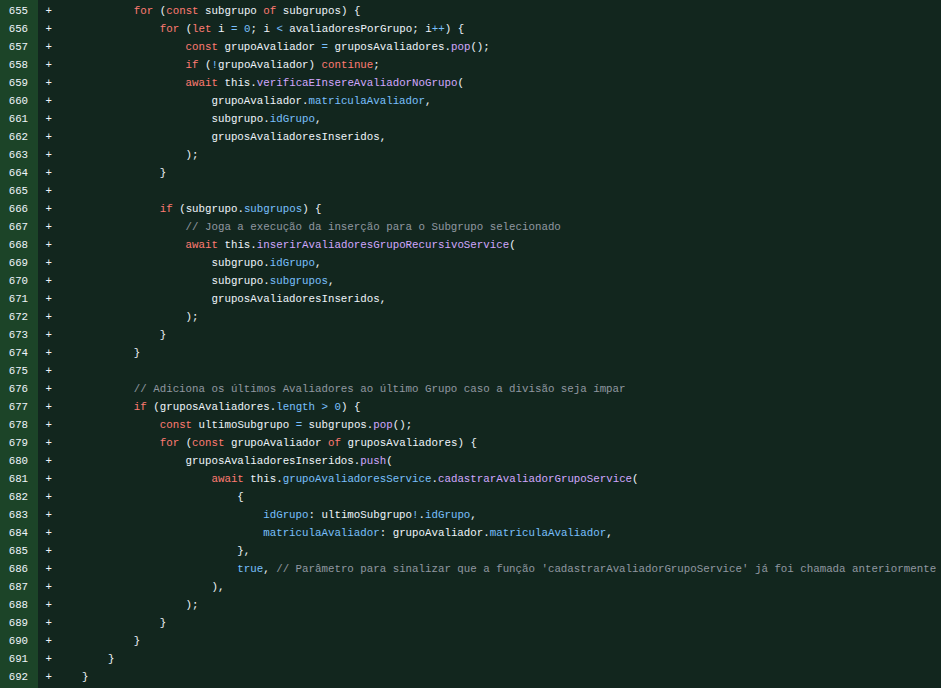
\includegraphics[scale=0.6]{./Imagens/tafeito/api/inserir_avaliador_grupo.png}
	\caption{Método que insere os Avaliadores nos Grupos}
	\label{fig:insere_avaliadores_grupos}
\end{figure}

Com isso, tanto a inserção quanto remoção de novos Avaliadores e a redivisão dos Grupos por meior da edição do TAF passam pelo mesmo tratamento recursivo, unificando os métodos de ambas funcionalidades, solucionando o \textit{bug} mencionado.

\subsection{Adicionar Militares por arquivo CSV}

Inicialmente, o projeto já se preocupava com a possibilidade de carregar dados para a aplicação de forma que o usuário não utilizasse a interface gráfica para cadastrar, um a um, os Militares presentes na Instituição. Pensando nisso, foi desenvolvido uma funcionalidade para carregar os usuários para o sistema por meio de planilhas em Excel, o qual corroborava com o objetivo almejado, afinal, seria possível criar um único arquivo contendo todas as informações para vários Militares e ser possível cadastrá-los por meio do \textit{upload} desta planilha.

% Pesquisar sobre a performance de arquivos CSV para migracao de dados
A proposta incial seria obter os dados dos Militares a partir de informações presentes no Banco de Dados da própria Instituição, o que seria necessário obter arquivos CSV para realizar essa injeção de dados. Esses arquivos são característicos por serem leves e fáceis de serem interpretados pelos humanos, por isso foi o tipo adotado à essa nova funcionalidade, sem contar na sua performance para migração de dados.

Para este trabalho, foi necessário envolver a API em Python, além de inserir novas opções no \textit{Frontend} para a inserção de arquivos CSV no cadastro de Militares, adotando algumas estratégias para sinalizar ao usuário qual tipo de arquivo estava sendo utilizado naquele momento da criação. Uma dessas estratégias consiste em modifiar o tipo do arquivo em todos os textos presentes na funcionalidade, seja para Excel (\autoref{fig:importar_militares_excel}) ou para CSV (\autoref{fig:importar_militares_csv}). Uma outra estratégia é permitir que o usuário realize o \textit{download} de um arquivo exemplo para preenchimento das informações com base no formato selecionado.

\begin{figure}[H]
	\centering
	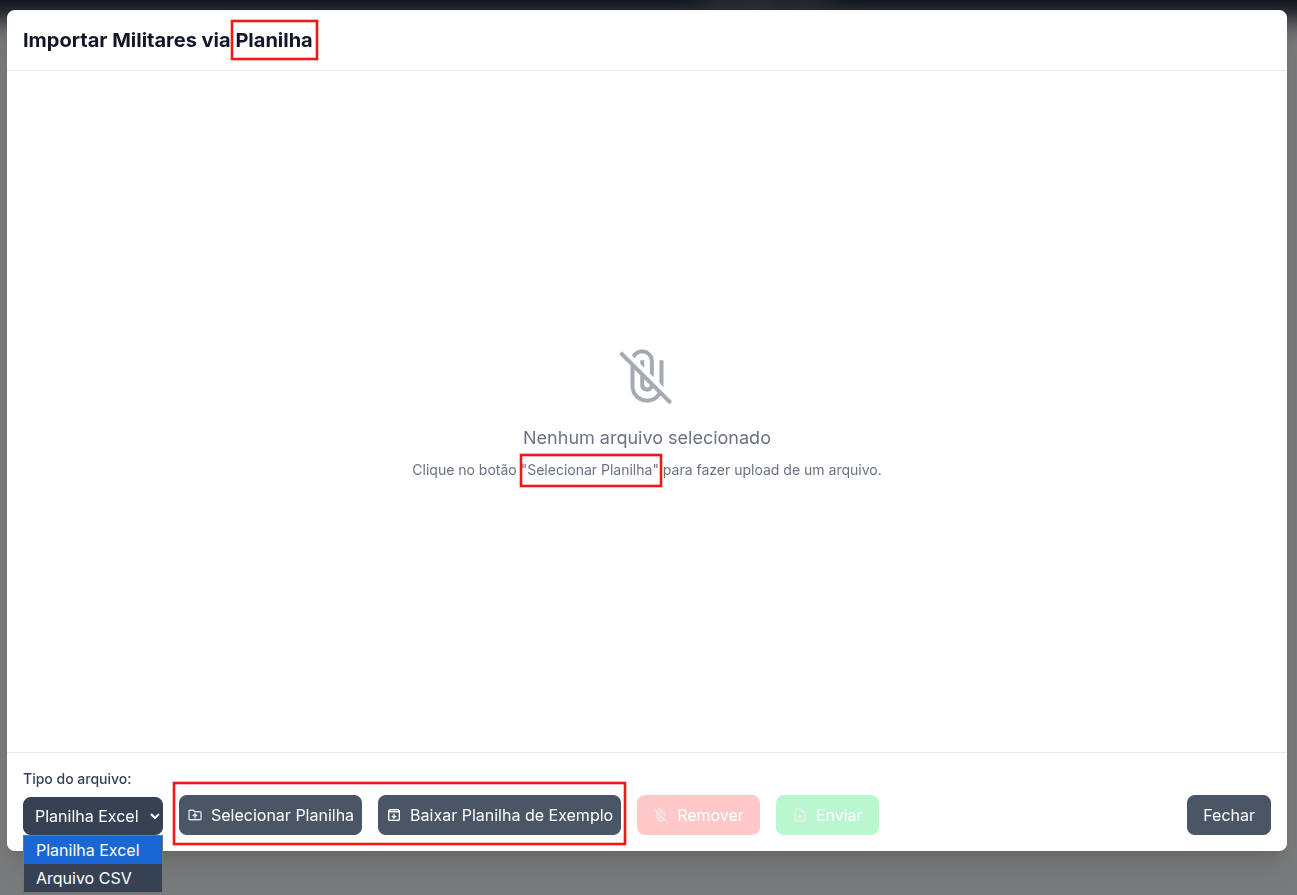
\includegraphics[scale=0.25]{./Imagens/tafeito/api/importar_militares_excel.png}
	\caption{Importar Militares com arquivos Excel}
	\label{fig:importar_militares_excel}
\end{figure}

\begin{figure}[H]
	\centering
	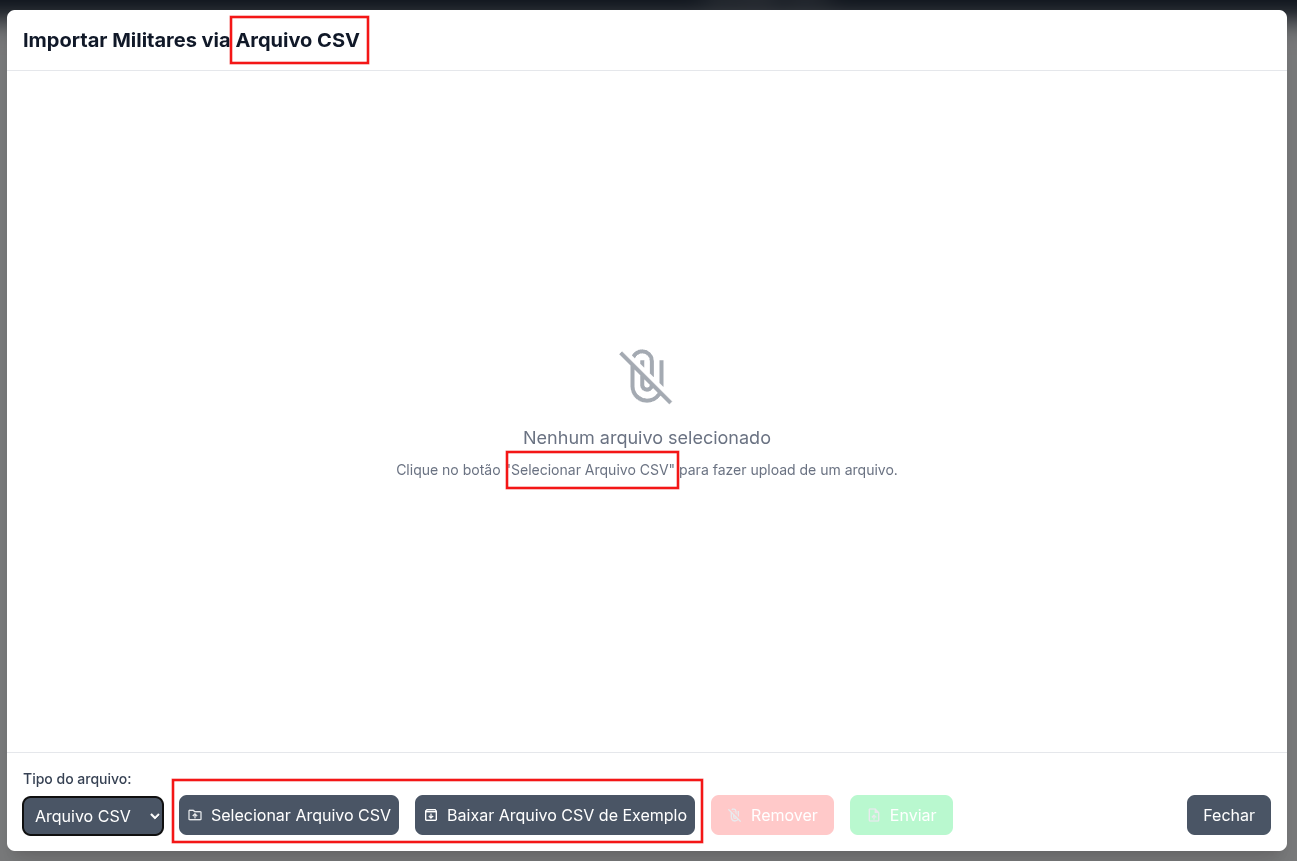
\includegraphics[scale=0.25]{./Imagens/tafeito/api/importar_militares_csv.png}
	\caption{Importar Militares com arquivos CSV}
	\label{fig:importar_militares_csv}
\end{figure}

Como citado anteriormente, foi envolvido a parte da API em Python, que é exclusiva ao gerenciamento desta funcionalidade de cadastro de Militares por arquivos (CSV e Excel) devido à facilidade de manipulação de dados utilizando esta linguagem. A biblioteca disponibilizada pelo Python para manipular arquios CSV foi mais que suficiente para o desenvolvimento desta feature, além disso, a existência de uma API em Python para o TAFeito traz avanços consideráveis em questão de manipulação de dados, o que propicia futuras demandas.

\subsection{Execução em Tempo Real}

\subsection{Edição do Nome da Unidade}

Como a aplicação permite que o usuário com maior papel a ser atuado (Coordenador) altere a maior parte das informações presentes no sistema, é viável que possíveis erros ocorridos devido às regras de negócio sejam relatados de forma clara e específica para não causar uma confusão ao mesmo. Desta forma, também é preferível que possíveis erros não voltados às regras de negócio, como incompatibilidade de dados, dados incompletos ou inexistentes, também sejam relatados ao usuário para que ele retome sua atenção à atividade executada. De fato, não há como tratar todas as ocorrências de erros existentes, afinal, o projeto possui uma alta complexidade em sua regra de negócio, porém, durante o desenvolvimento de POC II, houve uma preocupação em mitigar a maioria destes erros.

Ao final dos testes ocorridos em POC II, foi relatado um erro desconhecido ao usuário, pois não houve tratamento para ele. Este erro consistia na ação de edição do Nome de uma Unidade existente, onde retornava o erro "\textit{Cannot read properties of undefined (reading 'toString')}". Como uma Unidade possui uma relação com Militar, no caso, um Comandante, qualquer alteração no seu campo seria necessário enviar a matrícula deste Comandante, devido às verificações feitas pela API desenvolvida. O erro relatado consistia no envio da solicitação de edição, porém, sem a matrícula exigida.

Como solução, foi atribuída uma verificação para a existência dessa matrícula, além de inserí-la no \textit{payload} enviado à API, como relatado na \autoref{fig:editar_nome_unidade}.

\begin{figure}[H]
	\centering
	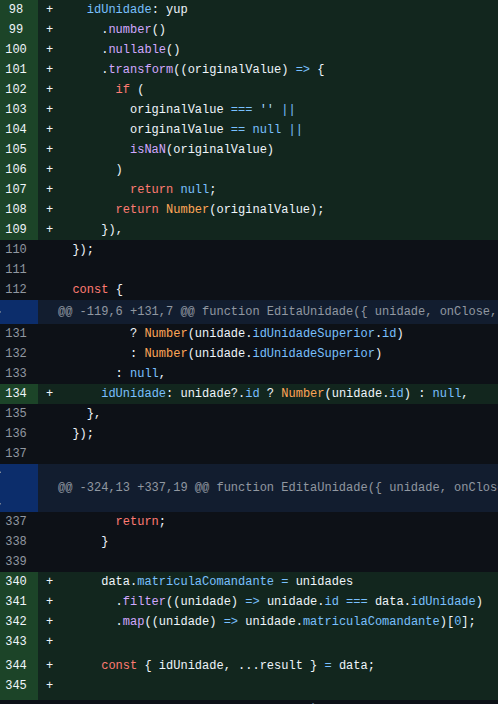
\includegraphics[scale=0.5]{./Imagens/tafeito/api/editar_nome_unidade.png}
	\caption{Edição do Nome da Unidade}
	\label{fig:editar_nome_unidade}
\end{figure}

\subsection{Remoção de Curso vinculado à Turma}

Voltando à uma das regras de negócio da aplicação, há o conceito de Turmas e Cursos. Essas Turmas são uma junção de Militares que almejam um objetivo em comum, seja conseguir entrar em uma Unidade, ou sejam recém-ingressos na Instituição. Já os Cursos, são criados para que ponha um signicado à uma Turma, por isso que há uma relação entre ambos. Como mencionado na \autoref{sub:exclusao_unidade_lotacao_militar}, erros de Banco de Dados jamais deverão ser direcionados ao usuário, pois eles não trazem significado, nem uma compreensão do por quê aconteceu aquele problema, devendo ser tratados durante o desenvolvimento da API. Portanto, como citado na subseção anterior, nem todos os erros são tratados durante o desenvolvimento.

O \textit{bug} relatado neste trabalho consiste na remoção de um Curso que possui uma Turma vinculada, ou seja, da perspectiva da regra de negócio esta ação deve ser impedida e tratada, mas, como relatado, não houve tratamento de sua execução. Por sorte, a resolução consiste em apenas uma verificação feita antes da remoção de um Curso, garantindo que ele não possui um relacionamento sequer com uma Turma, como pode ser visto na \autoref{fig:remocao_curso_turma}.

\begin{figure}[H]
	\centering
	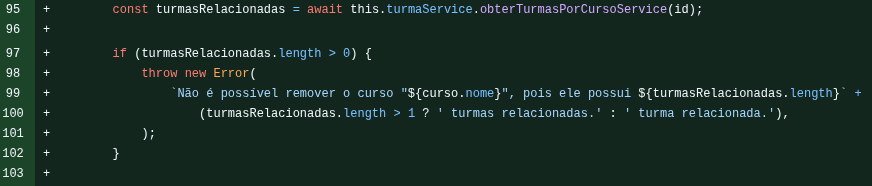
\includegraphics[scale=0.5]{./Imagens/tafeito/api/remocao_curso_com_turma.png}
	\caption{Remoção de Curso Atrelado à uma Turma}
	\label{fig:remocao_curso_turma}
\end{figure}

\subsection{Visualização do TAF pelo Avaliador}

Na aplicação, o perfil Avaliador possui um foco na execução dos TAFs na versão \textit{mobile}, mas nada impede dele também poder utilizar a visualização \textit{Web}. Pensando nisso que algumas funcionalidades foram liberadas para acesso, sendo a parte do TAF a principal delas, cuja visualização permite identificar quais militares estarão sendo avaliados e quais Avaliadores estarão presentes na avaliação, sendo estas ações também possíveis de serem feitas pelo aplicativo \textit{mobile}.

Um dos problemas relatados pela equipe de testes durante POC II foi que não era possível visualizar a composição do TAF a partir do perfil Avaliador, pois as informações de Grupos, Militares e Avaliadores estavam vazias e isso inviabilizava a proposta de exibição dos dados, mesmo o usuário acessando pela plataforma \textit{Web}. Pesquisando sobre o motivo, percebeu-se que os usuários com perfil Avaliador estavam recebendo erros de autorização, ou seja, eles não possuíam acesso ao \textit{endpoint} responsável por retornar os dados necessários à exibição, por isso, a solução foi bastante simples, pois bastaria apenas conceder esse acesso por meio de \textit{Roles} na própria API, retradado pela \autoref{fig:permissao_avaliador_grupos_taf}.

\begin{figure}[H]
	\centering
	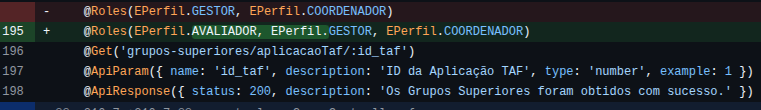
\includegraphics[scale=0.6]{./Imagens/tafeito/api/permissao_avaliadores_grupos_taf.png}
	\caption{\textit{Role} adicionada ao Perfil Avaliador}
	\label{fig:permissao_avaliador_grupos_taf}
\end{figure}

\subsection{Visualizações dos TAFs pelos Perfis Gestor, Coordenador e Avaliador}
